\documentclass[11pt,a4paper]{article}

\usepackage[margin=1in]{geometry}
\usepackage{amsmath,amssymb}
\usepackage{amsthm}
\newtheorem{proposition}{Proposition}
\newtheorem{corollary}{Corollary}
\newtheorem{theorem}{Theorem}
\newtheorem{conjecture}{Conjecture}
\usepackage{algorithm}
\usepackage{algpseudocodex}
\usepackage{booktabs}
\usepackage{longtable}
\usepackage{iftex}
\ifPDFTeX
  \usepackage[T1]{fontenc}
  \usepackage[utf8]{inputenc}
  \usepackage{lmodern}
\fi
\usepackage{microtype}
\usepackage{graphicx}
\usepackage[colorlinks=true, linkcolor=blue!50!black, citecolor=blue!50!black, urlcolor=blue!60!black, bookmarks=true, bookmarksopen=true, bookmarksnumbered=true]{hyperref}
\usepackage{bookmark}

\newcommand{\nbhd}[9]{%
  \begin{smallmatrix}
  #1 & #2 & #3 \\
  #4 & #5 & #6 \\
  #7 & #8 & #9
  \end{smallmatrix}
}
\newcommand{\F}[1]{f\!\left(#1\right)}
\newcommand{\sid}[1]{\texttt{sid:}\allowbreak\texttt{#1}}
% File paths: use \fpath instead of \texttt to allow breaks at / and _.
% \nolinkurl{} is provided by hyperref; arguments are literal characters
% (NO backslash-underscore escaping; just the raw path).
\newcommand{\fpath}[1]{\nolinkurl{#1}}
% Allow more flexible breaks inside paths and URLs.
\Urlmuskip=0mu plus 1mu\relax
% Allow URL/path line-breaks at hyphen and dot too (hyperref defaults
% break at / and _ but not - or .).
\makeatletter
\g@addto@macro\UrlBreaks{\do\-\do\.}
\makeatother
\newcommand{\torusparticles}[2]{%
  \begin{tikzpicture}[x=0.28cm,y=0.28cm,baseline=-0.6ex]
    \draw[step=1,black!60] (0,0) grid (4,4);
    \foreach \x/\y in {#1} {
      \fill[black] (\x,\y) rectangle ++(1,1);
    }
    \node[anchor=north,font=\scriptsize] at (2,-0.25) {#2};
  \end{tikzpicture}%
}
\newcommand{\torusholes}[2]{%
  \begin{tikzpicture}[x=0.28cm,y=0.28cm,baseline=-0.6ex]
    \fill[black!85] (0,0) rectangle (4,4);
    \draw[step=1,white!65] (0,0) grid (4,4);
    \foreach \x/\y in {#1} {
      \fill[white] (\x,\y) rectangle ++(1,1);
      \draw[black!60] (\x,\y) rectangle ++(1,1);
    }
    \node[anchor=north,font=\scriptsize,text=black] at (2,-0.25) {#2};
  \end{tikzpicture}%
}

\title{Enumeration and Classification of Number-Conserving Binary Moore-Neighborhood Cellular Automata}
\author{OpenAI Codex \and Witold Bo\l{}t}
\date{\today}

\begin{document}
\maketitle

\noindent\textit{Note.} The code, experiments, and manuscript were prepared with substantial
use of AI tools and have not yet been fully hand-verified by the human authors.

\bigskip
{\hypersetup{linkcolor=black}\tableofcontents}
\bigskip

\section{Problem Setting}

We study deterministic two-dimensional binary cellular automata (CAs) with the Moore
neighborhood
\[
\nbhd{x}{y}{z}{t}{u}{w}{a}{b}{c}
\]
and local update rule
\[
\F{\nbhd{x}{y}{z}{t}{u}{w}{a}{b}{c}} \in \{0,1\}.
\]

The truth table of \(f\) has \(2^9=512\) entries.  We index them by
\[
\nbhd{x}{y}{z}{t}{u}{w}{a}{b}{c}
\mapsto
256x+128y+64z+32t+16u+8w+4a+2b+c.
\]

Throughout, we restrict attention to \emph{double-legal} rules:
\[
\F{\nbhd{0}{0}{0}{0}{0}{0}{0}{0}{0}}=0,
\qquad
\F{\nbhd{1}{1}{1}{1}{1}{1}{1}{1}{1}}=1.
\]
Consequently the two boundary truth-table entries are fixed, and the actual search is over
\(x_1,\dots,x_{510}\).

Number-conserving cellular automata (NCCAs) have been studied for several decades as models of
particle transport and other conservative dynamics.  Foundational one-dimensional characterizations
were given by Boccara and Fuk\'s \cite{BoccaraFuks1998,BoccaraFuks2002}, while Durand,
Formenti, and R\'oka established a general decidability framework for number conservation
\cite{DurandFormentiRoka2003}.  Moreira showed that number conservation is also compatible with
intrinsic universality and broader state relabelings \cite{Moreira2003}.
The broader viewpoint of additive conserved quantities goes back at least to Hattori and Takesue
\cite{HattoriTakesue1991} and was later developed further by Pivato in a more general
conservation-law framework \cite{Pivato2002}.

\subsection{Related Work for the Two-Dimensional Case}

The literature most directly related to the present computations splits into two strands.
First, there is the Moore-neighborhood line: Imai and Tanimoto gave a construction method for
Moore-neighborhood NCCAs and, in particular, a sufficient condition tailored to this neighborhood
\cite{TanimotoImai2008}.  Second, there is a more extensive von Neumann-neighborhood line:
Tanimoto and Imai derived necessary and sufficient conditions for the two-dimensional von Neumann
case \cite{TanimotoImai2009}; Wolnik \emph{et al.} later generalized computationally tractable
conditions to arbitrary dimension for the range-one von Neumann neighborhood
\cite{WolnikDzedzejBaetensDeBaets2017}; Dzedzej \emph{et al.} used these conditions for exhaustive
enumeration of special two-dimensional classes, including binary, totalistic, and outer-totalistic
rules \cite{DzedzejWolnikNencaBaetensDeBaets2020}; and Dzedzej \emph{et al.} further specialized
the analysis to the rotation-symmetric von Neumann case \cite{DzedzejWolnikNencaBaetensDeBaets2021}.
For binary adjacent-cell dynamics, Wolnik and De Baets proved that all such von Neumann rules are
intrinsically one-dimensional, yielding exactly the identity, shifts, and traffic rules
\cite{WolnikDeBaets2019}.  A recent binary-specific structural result by Kong, Imai, and
Nakanishi introduces ``bundle pairs'' and ``bundle quads'' as organizing motifs for two-state
NCCAs \cite{KongImaiNakanishi2021}.

Taken together, these papers suggest that exhaustive two-dimensional NCCA enumeration has been
developed much further for the von Neumann neighborhood than for the binary Moore neighborhood.
The present computations therefore complement the literature by providing an exhaustive
classification for the binary Moore setting under a broad menu of additional functional
identities.

For the extra structural properties considered here, two further strands of literature are
particularly relevant.  First, conservative and monotone cellular automata have been studied
together in one dimension via particle representations by Moreira, Boccara, and Goles
\cite{MoreiraBoccaraGoles2004}, and Goles, Moreira, and Rapaport later showed that this combined
class has especially simple prediction complexity in the elementary setting
\cite{GolesMoreiraRapaport2011}.  Second, permutivity has a well-developed general theory; in
particular, Allouche and Skordev proved that every two-dimensional permutive cellular automaton
is conjugate to a one-sided shift \cite{AlloucheSkordev2003}.  This is directly relevant to our
site-permutive subclasses, which indeed collapse to rigid shifts in the number-conserving Moore
setting.

\section{Functional Identities Considered}

The starting point is a collection of functional identities written directly in terms of
\(f\).  Each identity is instantiated over all assignments of its free variables and converted
into a Boolean constraint over the truth-table entries.  The identity language supports
equality, disequality, and implication-style order relations:
\[
\F{\cdots}=\F{\cdots},\qquad
\F{\cdots}\neq \F{\cdots},\qquad
\F{\cdots}\le \F{\cdots},\qquad
\F{\cdots}\ge \F{\cdots},
\]
where the non-equality relations are restricted to Boolean atoms on each side.  The main base property is
number-conservation; all remaining identities are used as additional classifiers.  In spirit,
this identity-based pipeline plays a role analogous to the characterization theorems used in the
von Neumann literature \cite{TanimotoImai2009,WolnikDzedzejBaetensDeBaets2017,
DzedzejWolnikNencaBaetensDeBaets2020}, but here it is applied directly to the binary
Moore-neighborhood truth table.  It is also compatible with the broader conserved-quantity
viewpoint of \cite{HattoriTakesue1991,Pivato2002}, specialized here to the Boolean
state-sum invariant.

\subsection{Base Identity: Number-Conservation}

The number-conserving identity used in the computations is
\begingroup\small
\begin{align*}
\F{\nbhd{x}{y}{z}{t}{u}{w}{a}{b}{c}}
&=
x
+ \F{\nbhd{0}{y}{z}{0}{u}{w}{0}{b}{c}}
+ \F{\nbhd{0}{0}{y}{0}{0}{u}{0}{0}{b}} \\
&\quad
+ \F{\nbhd{0}{0}{0}{0}{y}{z}{0}{u}{w}}
+ \F{\nbhd{0}{0}{0}{0}{0}{y}{0}{0}{u}}
+ \F{\nbhd{0}{0}{0}{0}{0}{0}{0}{y}{z}} \\
&\quad
+ \F{\nbhd{0}{0}{0}{0}{0}{0}{0}{0}{y}}
+ \F{\nbhd{0}{0}{0}{t}{u}{w}{a}{b}{c}}
+ \F{\nbhd{0}{0}{0}{0}{t}{u}{0}{a}{b}} \\
&\quad
+ \F{\nbhd{0}{0}{0}{0}{0}{t}{0}{0}{a}}
+ \F{\nbhd{0}{0}{0}{0}{0}{0}{t}{u}{w}}
+ \F{\nbhd{0}{0}{0}{0}{0}{0}{0}{t}{u}} \\
&\quad
+ \F{\nbhd{0}{0}{0}{0}{0}{0}{0}{0}{t}}
- \F{\nbhd{0}{x}{y}{0}{t}{u}{0}{a}{b}}
- \F{\nbhd{0}{0}{x}{0}{0}{t}{0}{0}{a}} \\
&\quad
- \F{\nbhd{0}{0}{0}{x}{y}{z}{t}{u}{w}}
- \F{\nbhd{0}{0}{0}{0}{x}{y}{0}{t}{u}}
- \F{\nbhd{0}{0}{0}{0}{0}{x}{0}{0}{t}} \\
&\quad
- \F{\nbhd{0}{0}{0}{0}{0}{0}{x}{y}{z}}
- \F{\nbhd{0}{0}{0}{0}{0}{0}{0}{x}{y}}
- \F{\nbhd{0}{0}{0}{0}{0}{0}{0}{0}{x}} \\
&\quad
- \F{\nbhd{0}{0}{0}{0}{u}{w}{0}{b}{c}}
- \F{\nbhd{0}{0}{0}{0}{0}{u}{0}{0}{b}}
- \F{\nbhd{0}{0}{0}{0}{0}{0}{0}{u}{w}} \\
&\quad
- \F{\nbhd{0}{0}{0}{0}{0}{0}{0}{0}{u}}.
\end{align*}
\endgroup

\subsection{Symmetry Identities}

\paragraph{Rotations.}
\begin{align*}
\text{Rotation }90^\circ:\quad
\F{\nbhd{x}{y}{z}{t}{u}{w}{a}{b}{c}}
&=
\F{\nbhd{a}{t}{x}{b}{u}{y}{c}{w}{z}},\\
\text{Rotation }180^\circ:\quad
\F{\nbhd{x}{y}{z}{t}{u}{w}{a}{b}{c}}
&=
\F{\nbhd{c}{b}{a}{w}{u}{t}{z}{y}{x}}.
\end{align*}

\paragraph{Reflections.}
\begin{align*}
\text{Left-right:}\quad
\F{\nbhd{x}{y}{z}{t}{u}{w}{a}{b}{c}}
&=
\F{\nbhd{z}{y}{x}{w}{u}{t}{c}{b}{a}},\\
\text{Top-bottom:}\quad
\F{\nbhd{x}{y}{z}{t}{u}{w}{a}{b}{c}}
&=
\F{\nbhd{a}{b}{c}{t}{u}{w}{x}{y}{z}},\\
\text{Main diagonal:}\quad
\F{\nbhd{x}{y}{z}{t}{u}{w}{a}{b}{c}}
&=
\F{\nbhd{x}{t}{a}{y}{u}{b}{z}{w}{c}},\\
\text{Anti-diagonal:}\quad
\F{\nbhd{x}{y}{z}{t}{u}{w}{a}{b}{c}}
&=
\F{\nbhd{c}{w}{z}{b}{u}{y}{a}{t}{x}}.
\end{align*}

The combined families are defined by conjunction:
\begin{itemize}
\item axis-reflection symmetric \(=\) left-right \(+\) top-bottom;
\item diagonal-reflection symmetric \(=\) main-diagonal \(+\) anti-diagonal;
\item isotropic non-totalistic \(=\) rotation \(90^\circ\) \(+\) left-right reflection.
\end{itemize}

\subsection{Complement Symmetry}

Black/white symmetry is expressed by
\[
\F{\nbhd{x}{y}{z}{t}{u}{w}{a}{b}{c}}
=
1-\F{\nbhd{1-x}{1-y}{1-z}{1-t}{1-u}{1-w}{1-a}{1-b}{1-c}}.
\]

\subsection{Neighborhood-Irrelevance Identities}

\paragraph{Center-blind.}
\[
\F{\nbhd{x}{y}{z}{t}{u}{w}{a}{b}{c}}
=
\F{\nbhd{x}{y}{z}{t}{1-u}{w}{a}{b}{c}}.
\]

\paragraph{Von Neumann embedded family.}
\begin{align*}
\F{\nbhd{x}{y}{z}{t}{u}{w}{a}{b}{c}}
&=
\F{\nbhd{1-x}{y}{z}{t}{u}{w}{a}{b}{c}},\\
\F{\nbhd{x}{y}{z}{t}{u}{w}{a}{b}{c}}
&=
\F{\nbhd{x}{y}{1-z}{t}{u}{w}{a}{b}{c}},\\
\F{\nbhd{x}{y}{z}{t}{u}{w}{a}{b}{c}}
&=
\F{\nbhd{x}{y}{z}{t}{u}{w}{1-a}{b}{c}},\\
\F{\nbhd{x}{y}{z}{t}{u}{w}{a}{b}{c}}
&=
\F{\nbhd{x}{y}{z}{t}{u}{w}{a}{b}{1-c}}.
\end{align*}

\paragraph{Diagonal-only family.}
\begin{align*}
\F{\nbhd{x}{y}{z}{t}{u}{w}{a}{b}{c}}
&=
\F{\nbhd{x}{1-y}{z}{t}{u}{w}{a}{b}{c}},\\
\F{\nbhd{x}{y}{z}{t}{u}{w}{a}{b}{c}}
&=
\F{\nbhd{x}{y}{z}{1-t}{u}{w}{a}{b}{c}},\\
\F{\nbhd{x}{y}{z}{t}{u}{w}{a}{b}{c}}
&=
\F{\nbhd{x}{y}{z}{t}{u}{1-w}{a}{b}{c}},\\
\F{\nbhd{x}{y}{z}{t}{u}{w}{a}{b}{c}}
&=
\F{\nbhd{x}{y}{z}{t}{u}{w}{a}{1-b}{c}}.
\end{align*}

We also refer to this same family as the \emph{diagonal von Neumann embedded} class, because it
is the exact diagonal analogue of the embedded von Neumann restriction: the rule depends only on
the five sites \(\{x,z,u,a,c\}\).

\subsection{Order And Permutivity Identities}

\paragraph{Monotone family.}
Monotonicity is expressed coordinatewise.  For example:
\begin{align*}
\F{\nbhd{0}{y}{z}{t}{u}{w}{a}{b}{c}}
&\le
\F{\nbhd{1}{y}{z}{t}{u}{w}{a}{b}{c}},\\
\F{\nbhd{x}{0}{z}{t}{u}{w}{a}{b}{c}}
&\le
\F{\nbhd{x}{1}{z}{t}{u}{w}{a}{b}{c}},\\
\F{\nbhd{x}{y}{z}{t}{u}{w}{a}{b}{0}}
&\le
\F{\nbhd{x}{y}{z}{t}{u}{w}{a}{b}{1}},
\end{align*}
and similarly for the remaining six sites.  Thus flipping any single neighborhood bit from
\(0\) to \(1\) cannot decrease the output.

\paragraph{Antitone family.}
Antitonicity reverses the inequalities:
\[
\F{\nbhd{0}{y}{z}{t}{u}{w}{a}{b}{c}}
\ge
\F{\nbhd{1}{y}{z}{t}{u}{w}{a}{b}{c}},
\]
and similarly for the remaining eight sites.

\paragraph{Partial monotonicity families.}
The same syntax gives one-coordinate and subset-restricted variants.  For example:
\begin{align*}
\text{center-monotone:}\quad
\F{\nbhd{x}{y}{z}{t}{0}{w}{a}{b}{c}}
&\le
\F{\nbhd{x}{y}{z}{t}{1}{w}{a}{b}{c}},\\
\text{center-antitone:}\quad
\F{\nbhd{x}{y}{z}{t}{0}{w}{a}{b}{c}}
&\ge
\F{\nbhd{x}{y}{z}{t}{1}{w}{a}{b}{c}},\\
\text{outer-monotone:}\quad
\F{\nbhd{0}{y}{z}{t}{u}{w}{a}{b}{c}}
&\le
\F{\nbhd{1}{y}{z}{t}{u}{w}{a}{b}{c}},\\
\text{orthogonal-monotone:}\quad
\F{\nbhd{x}{0}{z}{t}{u}{w}{a}{b}{c}}
&\le
\F{\nbhd{x}{1}{z}{t}{u}{w}{a}{b}{c}},\\
\text{diagonal-monotone:}\quad
\F{\nbhd{0}{y}{z}{t}{u}{w}{a}{b}{c}}
&\le
\F{\nbhd{1}{y}{z}{t}{u}{w}{a}{b}{c}}.
\end{align*}
The full files contain the obvious coordinatewise generators for the chosen subset of sites.

\paragraph{Center-permutive family.}
Center permutivity is captured by the Boolean disequality
\[
\F{\nbhd{x}{y}{z}{t}{0}{w}{a}{b}{c}}
\neq
\F{\nbhd{x}{y}{z}{t}{1}{w}{a}{b}{c}}.
\]
For every fixed outer neighborhood, changing the center cell flips the output.  This is a local
permutivity condition in the standard CA sense \cite{AlloucheSkordev2003}.

\paragraph{Non-central site-permutive families.}
The same construction is used for each of the eight outer sites.  For example:
\begin{align*}
\text{\(x\)-permutive:}\quad
\F{\nbhd{0}{y}{z}{t}{u}{w}{a}{b}{c}}
&\neq
\F{\nbhd{1}{y}{z}{t}{u}{w}{a}{b}{c}},\\
\text{\(y\)-permutive:}\quad
\F{\nbhd{x}{0}{z}{t}{u}{w}{a}{b}{c}}
&\neq
\F{\nbhd{x}{1}{z}{t}{u}{w}{a}{b}{c}},
\end{align*}
and analogously for \(z,t,w,a,b,c\).  Again, these are local permutivity conditions in the
sense of \cite{AlloucheSkordev2003}.

\subsection{Count-Based and Semi-Totalistic Identities}

\paragraph{Outer-totalistic / Life-like.}
These families are identical in the binary Moore-neighborhood setting and are generated by
\begin{align*}
\F{\nbhd{x}{y}{z}{t}{u}{w}{a}{b}{c}} &= \F{\nbhd{y}{x}{z}{t}{u}{w}{a}{b}{c}},\\
\F{\nbhd{x}{y}{z}{t}{u}{w}{a}{b}{c}} &= \F{\nbhd{x}{z}{y}{t}{u}{w}{a}{b}{c}},\\
\F{\nbhd{x}{y}{z}{t}{u}{w}{a}{b}{c}} &= \F{\nbhd{x}{y}{z}{w}{u}{t}{a}{b}{c}},\\
\F{\nbhd{x}{y}{z}{t}{u}{w}{a}{b}{c}} &= \F{\nbhd{x}{y}{z}{t}{u}{a}{w}{b}{c}},\\
\F{\nbhd{x}{y}{z}{t}{u}{w}{a}{b}{c}} &= \F{\nbhd{x}{y}{z}{t}{u}{w}{b}{a}{c}},\\
\F{\nbhd{x}{y}{z}{t}{u}{w}{a}{b}{c}} &= \F{\nbhd{x}{y}{z}{t}{u}{w}{a}{c}{b}},\\
\F{\nbhd{x}{y}{z}{t}{u}{w}{a}{b}{c}} &= \F{\nbhd{t}{y}{z}{x}{u}{w}{a}{b}{c}}.
\end{align*}

\paragraph{Totalistic.}
\begin{align*}
\F{\nbhd{x}{y}{z}{t}{u}{w}{a}{b}{c}} &= \F{\nbhd{y}{x}{z}{t}{u}{w}{a}{b}{c}},\\
\F{\nbhd{x}{y}{z}{t}{u}{w}{a}{b}{c}} &= \F{\nbhd{x}{z}{y}{t}{u}{w}{a}{b}{c}},\\
\F{\nbhd{x}{y}{z}{t}{u}{w}{a}{b}{c}} &= \F{\nbhd{x}{y}{t}{z}{u}{w}{a}{b}{c}},\\
\F{\nbhd{x}{y}{z}{t}{u}{w}{a}{b}{c}} &= \F{\nbhd{x}{y}{z}{u}{t}{w}{a}{b}{c}},\\
\F{\nbhd{x}{y}{z}{t}{u}{w}{a}{b}{c}} &= \F{\nbhd{x}{y}{z}{t}{w}{u}{a}{b}{c}},\\
\F{\nbhd{x}{y}{z}{t}{u}{w}{a}{b}{c}} &= \F{\nbhd{x}{y}{z}{t}{u}{a}{w}{b}{c}},\\
\F{\nbhd{x}{y}{z}{t}{u}{w}{a}{b}{c}} &= \F{\nbhd{x}{y}{z}{t}{u}{w}{b}{a}{c}},\\
\F{\nbhd{x}{y}{z}{t}{u}{w}{a}{b}{c}} &= \F{\nbhd{x}{y}{z}{t}{u}{w}{a}{c}{b}}.
\end{align*}

\paragraph{Orthogonal/diagonal semi-totalistic.}
\begin{align*}
\F{\nbhd{x}{y}{z}{t}{u}{w}{a}{b}{c}} &= \F{\nbhd{z}{y}{x}{t}{u}{w}{a}{b}{c}},\\
\F{\nbhd{x}{y}{z}{t}{u}{w}{a}{b}{c}} &= \F{\nbhd{x}{y}{a}{t}{u}{w}{z}{b}{c}},\\
\F{\nbhd{x}{y}{z}{t}{u}{w}{a}{b}{c}} &= \F{\nbhd{x}{y}{z}{t}{u}{w}{c}{b}{a}},\\
\F{\nbhd{x}{y}{z}{t}{u}{w}{a}{b}{c}} &= \F{\nbhd{x}{t}{z}{y}{u}{w}{a}{b}{c}},\\
\F{\nbhd{x}{y}{z}{t}{u}{w}{a}{b}{c}} &= \F{\nbhd{x}{y}{z}{w}{u}{t}{a}{b}{c}},\\
\F{\nbhd{x}{y}{z}{t}{u}{w}{a}{b}{c}} &= \F{\nbhd{x}{y}{z}{t}{u}{b}{a}{w}{c}}.
\end{align*}

\paragraph{Orthogonal-totalistic.}
Diagonal irrelevance together with orthogonal permutation invariance:
\begin{align*}
\F{\nbhd{x}{y}{z}{t}{u}{w}{a}{b}{c}} &= \F{\nbhd{1-x}{y}{z}{t}{u}{w}{a}{b}{c}},\\
\F{\nbhd{x}{y}{z}{t}{u}{w}{a}{b}{c}} &= \F{\nbhd{x}{y}{1-z}{t}{u}{w}{a}{b}{c}},\\
\F{\nbhd{x}{y}{z}{t}{u}{w}{a}{b}{c}} &= \F{\nbhd{x}{y}{z}{t}{u}{w}{1-a}{b}{c}},\\
\F{\nbhd{x}{y}{z}{t}{u}{w}{a}{b}{c}} &= \F{\nbhd{x}{y}{z}{t}{u}{w}{a}{b}{1-c}},\\
\F{\nbhd{x}{y}{z}{t}{u}{w}{a}{b}{c}} &= \F{\nbhd{x}{t}{z}{y}{u}{w}{a}{b}{c}},\\
\F{\nbhd{x}{y}{z}{t}{u}{w}{a}{b}{c}} &= \F{\nbhd{x}{y}{z}{w}{u}{t}{a}{b}{c}},\\
\F{\nbhd{x}{y}{z}{t}{u}{w}{a}{b}{c}} &= \F{\nbhd{x}{y}{z}{t}{u}{b}{a}{w}{c}}.
\end{align*}

\paragraph{Diagonal-totalistic.}
Orthogonal irrelevance together with diagonal permutation invariance:
\begin{align*}
\F{\nbhd{x}{y}{z}{t}{u}{w}{a}{b}{c}} &= \F{\nbhd{x}{1-y}{z}{t}{u}{w}{a}{b}{c}},\\
\F{\nbhd{x}{y}{z}{t}{u}{w}{a}{b}{c}} &= \F{\nbhd{x}{y}{z}{1-t}{u}{w}{a}{b}{c}},\\
\F{\nbhd{x}{y}{z}{t}{u}{w}{a}{b}{c}} &= \F{\nbhd{x}{y}{z}{t}{u}{1-w}{a}{b}{c}},\\
\F{\nbhd{x}{y}{z}{t}{u}{w}{a}{b}{c}} &= \F{\nbhd{x}{y}{z}{t}{u}{w}{a}{1-b}{c}},\\
\F{\nbhd{x}{y}{z}{t}{u}{w}{a}{b}{c}} &= \F{\nbhd{z}{y}{x}{t}{u}{w}{a}{b}{c}},\\
\F{\nbhd{x}{y}{z}{t}{u}{w}{a}{b}{c}} &= \F{\nbhd{x}{y}{a}{t}{u}{w}{z}{b}{c}},\\
\F{\nbhd{x}{y}{z}{t}{u}{w}{a}{b}{c}} &= \F{\nbhd{x}{y}{z}{t}{u}{w}{c}{b}{a}}.
\end{align*}

\subsection{Relations Among the Properties}

Several of the studied families are not independent.  The most important logical containments
used in interpreting the results are:
\begin{enumerate}
\item \textbf{Life-like \(=\) outer-totalistic.}
      In the binary Moore-neighborhood setting these names describe the same class.
\item \textbf{Totalistic \(\Rightarrow\) outer-totalistic.}
      Dependence only on the total number of live cells clearly implies dependence only on
      \(u\) and the number of live outer neighbors.
\item \textbf{Outer-totalistic \(\Rightarrow\) orthogonal/diagonal semi-totalistic.}
      If only the total outer population matters, then the separate orthogonal and diagonal
      multisets certainly do not matter.
\item \textbf{Totalistic \(\Rightarrow\) orthogonal-totalistic and diagonal-totalistic.}
      A rule depending only on the total neighborhood population automatically depends only on
      \(u\) together with either the orthogonal or diagonal counts.
\item \textbf{Diagonal-totalistic \(\Rightarrow\) diagonal-only.}
      The former already enforces irrelevance of all orthogonal sites.
\item \textbf{Orthogonal-totalistic \(\Rightarrow\) von Neumann.}
      The former already enforces irrelevance of all diagonal sites.
\item \textbf{Isotropic non-totalistic \(\Rightarrow\) rotation \(90^\circ\), rotation \(180^\circ\),}
      \textbf{and all four reflections.}
      This follows because the isotropic non-totalistic class is defined by the full dihedral
      symmetry group \(D_4\).
\item \textbf{Rotation \(90^\circ\) \(\Rightarrow\) rotation \(180^\circ\).}
\item \textbf{Axis-reflection symmetric \(\Rightarrow\) rotation \(180^\circ\).}
      The composition of left-right and top-bottom reflections is a half-turn.
\item \textbf{Diagonal-reflection symmetric \(\Rightarrow\) rotation \(180^\circ\).}
      The composition of the two diagonal reflections is also a half-turn.
\item \textbf{Outer-totalistic \(\Rightarrow\) isotropic non-totalistic.}
      Outer-totalistic rules are invariant under all permutations of the eight outer sites and
      therefore under every geometric symmetry of the Moore neighborhood.
\item \textbf{Hence totalistic \(\Rightarrow\) outer-totalistic \(\Rightarrow\) isotropic non-totalistic.}
\item \textbf{Monotone \(\Rightarrow\) center-monotone, outer-monotone, orthogonal-monotone, and diagonal-monotone.}
\item \textbf{Outer-monotone \(\Rightarrow\) orthogonal-monotone and diagonal-monotone.}
\item \textbf{Center-permutive \(\Rightarrow\) not center-blind.}
      If flipping \(u\) always flips the output, then the rule certainly depends on \(u\).
\item \textbf{Antitone is incompatible with double legality.}
      Since \(f(\mathbf{0})=0\) and \(f(\mathbf{1})=1\), a globally antitone rule would require
      \(0=f(\mathbf{0}) \ge f(\mathbf{1})=1\), which is impossible.
\end{enumerate}

These containments are consistent with the computed counts.  For example, the unique
outer-totalistic rule is automatically also Life-like, orthogonal/diagonal semi-totalistic,
rotation-symmetric, and isotropic non-totalistic.

\section{Algorithmic Pipeline}

\subsection{From Functional Identities to Linear Equations}

The generator reads a small identity language in which expressions are affine combinations of
variables, constants, and terms of the form \(f(\cdots)\).  Relations may be `\(=\)`, `\(\neq\)`,
`\(\le\)`, or `\(\ge\)`, with the latter three restricted to Boolean atoms on each side.  For each identity:
\begin{enumerate}
\item the free variables are detected automatically;
\item the identity is instantiated over all Boolean assignments of those variables;
\item each \(f(\cdots)\) call is mapped to a truth-table variable \(x_k\);
\item the identity is simplified into either an affine equality, an affine parity row, or an implication between LUT entries.
\end{enumerate}

This transformation is summarized in Algorithm~\ref{alg:generator-pipeline}.

\begin{algorithm}[t]
\caption{Functional identities to sparse Boolean constraints}
\label{alg:generator-pipeline}
\begin{algorithmic}[1]
\State parse the identity specification file
\State initialize the constraint set \(\mathcal{C} \gets \varnothing\)
\For{each identity \(I\) in the specification}
  \State detect the free Boolean variables of \(I\)
  \For{each Boolean assignment \(\alpha\) of those free variables}
    \State substitute \(\alpha\) into both sides of \(I\)
    \State rewrite every \(\F{\cdots}\) call as the corresponding LUT variable \(x_k\)
    \State simplify constants and collect like terms
    \If{\(I\) is an equality}
      \State emit an affine row \(\sum_j a_j x_j = b\)
    \ElsIf{\(I\) is a disequality between Boolean atoms}
      \State emit the parity relation \(x_i + x_j = 1\)
    \Else
      \State emit the implication-style constraint \(x_i \le x_j\) or \(x_i \ge x_j\)
    \EndIf
    \State insert the normalized constraint into \(\mathcal{C}\)
  \EndFor
\EndFor
\State deduplicate all constraints in \(\mathcal{C}\)
\State substitute the fixed boundary values \(x_0 = 0\) and \(x_{511} = 1\)
\State remove tautologies and detect immediate contradictions
\State write the sparse model and optional matrix/debug views
\end{algorithmic}
\end{algorithm}

The resulting equations are deduplicated.  Finally the two fixed entries
\[
x_0=0,\qquad x_{511}=1
\]
are substituted out, leaving a Boolean linear system in the \(510\) unknowns
\[
x_1,\dots,x_{510}.
\]

\subsection{Base Solver}

The optimized solver enumerates all Boolean solutions of the base system.  The main ideas are:
\begin{enumerate}
\item sparse row storage with flattened coefficient arrays;
\item depth-first search over \(x_1,\dots,x_{510}\);
\item row-feasibility bounds from the current partial assignment;
\item forced-assignment propagation when a row leaves only one feasible value for a variable;
\item reversible trails for assignments and row-state updates instead of recomputation;
\item OpenMP task splitting near the top of the search tree, followed by sequential descent.
\end{enumerate}

For each row \(r\), the solver maintains the current residual target together with the
remaining positive and negative coefficient sums.  A branch is cut immediately when the row
target falls outside the feasible interval.  This provides the main pruning mechanism.

\subsection{Implementation-Level Summary}

The equation generator is implemented in
\texttt{generate\_functional\_equation\_system.py}.  It parses the functional-identity input,
instantiates all Boolean assignments of the free variables, rewrites each \(\F{\cdots}\) call
to the corresponding LUT variable, and emits the sparse linear system used by the solver.
Conceptually, this bridges the gap between explicit Moore-neighborhood functional identities of
the type considered by Imai and Tanimoto \cite{TanimotoImai2008} and the exhaustive
computer-assisted enumeration strategy used in the more recent von Neumann studies
\cite{DzedzejWolnikNencaBaetensDeBaets2020,DzedzejWolnikNencaBaetensDeBaets2021}.

The optimized enumerator is implemented in \texttt{solve\_omp\_opt.cpp}.  The main code paths are:
\begin{itemize}
\item \texttt{load\_model}: parse the sparse integer system and build flattened row storage;
\item \texttt{assign\_var}, \texttt{propagate}, \texttt{undo}: maintain the reversible state of
      a partial assignment;
\item \texttt{compile\_property}: reduce an additional property system into fixed-value checks,
      affine binary relations, implication checks, and residual generic rows;
\item \texttt{dfs\_task} and \texttt{dfs\_seq}: perform the OpenMP task-parallel and sequential
      parts of the search;
\item \texttt{classify\_solution} and \texttt{record\_solution}: compute the property bit mask,
      accumulate exact-mask counts, and optionally write the packed rule vector to the output
      catalog.
\end{itemize}

At a high level, the solver executes the procedure shown in Algorithm~\ref{alg:solver-pipeline}.

\begin{algorithm}[t]
\caption{Enumeration and classification pipeline}
\label{alg:solver-pipeline}
\begin{algorithmic}[1]
\State build the base system from the functional identities
\State substitute \(x_0 = 0\) and \(x_{511} = 1\)
\State load the sparse base matrix \(M\)
\For{each additional property \(P_i\)}
  \State compile \(P_i\) into fast checks \(C_i\)
\EndFor
\State initialize the exact-mask counters
\Procedure{Explore}{$\sigma$}
  \If{any row of \(M\) is infeasible under \(\sigma\)}
    \State \Return
  \EndIf
  \State propagate all forced assignments implied by near-tight rows
  \If{all LUT variables are assigned in \(\sigma\)}
    \State \(m \gets 0\)
    \For{each compiled property check set \(C_i\)}
      \If{\(C_i\) accepts the complete LUT}
        \State set bit \(i\) in \(m\)
      \EndIf
    \EndFor
    \State increment \(\texttt{exact\_mask\_counts}[m]\)
    \If{output is enabled and \((m \neq 0)\) or all masks are requested}
      \State write \([\text{mask bytes}][\text{packed LUT bytes}]\)
    \EndIf
    \State \Return
  \EndIf
  \State choose the next variable \(x_k\) from \(\texttt{var\_order}\)
  \For{each \(v \in \{0,1\}\)}
    \State assign \(x_k \gets v\) using reversible row updates
    \State \Call{Explore}{extended assignment}
    \State undo the assignment trail
  \EndFor
\EndProcedure
\State launch OpenMP tasks for the top levels of \Call{Explore}{\(\sigma_0\)}
\end{algorithmic}
\end{algorithm}

The row-feasibility test used inside \texttt{assign\_var} and \texttt{propagate} is purely
interval based.  For each row \(r\), the solver maintains
\[
\text{target}_r,\qquad
\text{pos\_rem}_r,\qquad
\text{neg\_rem}_r,
\]
where \(\text{pos\_rem}_r\) and \(\text{neg\_rem}_r\) are the sums of the still-unassigned
positive and negative coefficients in that row.  The current branch can survive only if
\[
\text{neg\_rem}_r \le \text{target}_r \le \text{pos\_rem}_r.
\]
If setting an unassigned variable to \(0\) or to \(1\) would violate this interval, the other
value is forced immediately.  This very cheap bound test is the central mechanism that makes the
full enumeration practical.

\subsection{Property Matcher and Bit Masks}

Additional properties are not used for search pruning.  Instead, every complete solution of the
base system is classified against each additional property system.

Each property system is compiled into four kinds of checks:
\begin{enumerate}
\item fixed-value checks \(x_i=0\) or \(x_i=1\);
\item binary affine relations \(x_i=x_j\) or \(x_i=1-x_j\);
\item implication checks \(x_i \Rightarrow x_j\), equivalently \(x_i \le x_j\);
\item residual generic rows for constraints that cannot be reduced to the previous three forms.
\end{enumerate}

After a full base solution is found, the classifier evaluates all additional properties and
stores the result in a bit mask
\[
m \in \{0,1\}^{N},
\]
where \(N\) is the number of additional property families.  Bit \(i\) is set iff the current
base solution also satisfies property \(i\).

\subsection{Catalog Construction}

The final output is:
\begin{enumerate}
\item the total number of number-conserving rules;
\item counts for each individual property;
\item counts for each exact property-mask combination;
\item a compact binary catalog of all rules with nonzero masks, where each record stores
      the property bit mask together with the packed \(510\)-bit rule vector.
\end{enumerate}

In the current dataset, the union of all nonzero-mask classes contains \(133713\) rules.  These
are exactly the number-conserving rules satisfying at least one of the additional property
families listed above.  For downstream analysis, the checked-in JSON catalog now also assigns
two additional identifiers to every rule:
\begin{itemize}
\item a \emph{stable index}, obtained by sorting the catalog lexicographically by LUT;
\item a \emph{stable identifier}, namely the SHA-256 digest of the \(128\)-hex LUT string.
\end{itemize}
This is important because the raw binary emission order is not intrinsically stable under
parallel solving.  Any purely positional identifier inherited from write order should therefore
be treated as a transient implementation detail rather than as a permanent rule name.  In the
discussion below, when individual rules need to be named explicitly, we use short
\sid{\dots} prefixes of the stable SHA-256 LUT identifier.

\section{Results}

The corrected full enumeration found
\[
147{,}309{,}433
\]
number-conserving binary Moore-neighborhood rules.

For interpretation it is helpful to split the property families into three regimes: empty
classes, singleton classes, and genuinely nontrivial classes with more than one rule.

\subsection{Classes With Count \(=0\)}

\begin{table}[htbp]
\centering
\begin{tabular}{@{}lr@{}}
\toprule
Property family & Count \\
\midrule
Antitone & 0 \\
Totalistic & 0 \\
\bottomrule
\end{tabular}
\caption{Empty subclasses inside the number-conserving Moore-neighborhood class.}
\label{tab:counts-zero}
\end{table}

These two empty classes fail for different reasons.

For the antitone family, emptiness is essentially forced by the double-legal boundary
conditions: a globally antitone rule must satisfy
\[
f(\mathbf{0}) \ge f(\mathbf{1}),
\]
but double legality imposes \(f(\mathbf{0})=0\) and \(f(\mathbf{1})=1\), giving the
contradiction \(0 \ge 1\).

For the totalistic family, there is no such immediate logical contradiction.  Rather, the
exhaustive computation shows that number conservation is too rigid to coexist with full
dependence only on the total \(3\times 3\) population.  The unique outer-totalistic rule is
already the identity, and the stronger totalistic constraint eliminates even that possibility.

\subsection{Classes With Count \(=1\)}

\begin{table}[htbp]
\centering
\begin{tabular}{@{}lr@{}}
\toprule
Property family & Count \\
\midrule
Axis reflection symmetric & 1 \\
A-permutive & 1 \\
B-permutive & 1 \\
C-permutive & 1 \\
Center permutive & 1 \\
Diagonal reflection symmetric & 1 \\
Diagonal totalistic & 1 \\
Isotropic non-totalistic & 1 \\
Life-like & 1 \\
Orthogonal/diagonal semi-totalistic & 1 \\
Orthogonal totalistic & 1 \\
Outer totalistic & 1 \\
T-permutive & 1 \\
W-permutive & 1 \\
X-permutive & 1 \\
Y-permutive & 1 \\
Z-permutive & 1 \\
\bottomrule
\end{tabular}
\caption{Singleton subclasses inside the number-conserving Moore-neighborhood class.}
\label{tab:counts-one}
\end{table}

Most singleton classes reduce to the identity rule
\begin{itemize}
\item axis-reflection symmetric,
\item diagonal-reflection symmetric,
\item diagonal-totalistic,
\item isotropic non-totalistic,
\item Life-like,
\item center-permutive,
\item orthogonal/diagonal semi-totalistic,
\item orthogonal-totalistic,
\item outer-totalistic
\end{itemize}
and their unique element is the \emph{identity rule}
\[
\F{\nbhd{x}{y}{z}{t}{u}{w}{a}{b}{c}} = u.
\]
Its dynamics are trivial: every configuration is a fixed point, so the global CA leaves the
entire lattice unchanged at every time step.

The eight non-central site-permutive singleton classes are the only exception.  Each one contains
the corresponding one-step shift:
\begin{align*}
x\text{-permutive} &\Longleftrightarrow f=x, &
y\text{-permutive} &\Longleftrightarrow f=y, \\
z\text{-permutive} &\Longleftrightarrow f=z, &
t\text{-permutive} &\Longleftrightarrow f=t, \\
w\text{-permutive} &\Longleftrightarrow f=w, &
a\text{-permutive} &\Longleftrightarrow f=a, \\
b\text{-permutive} &\Longleftrightarrow f=b, &
c\text{-permutive} &\Longleftrightarrow f=c.
\end{align*}
Thus the singleton regime is still dominated by extremely simple dynamics: either the identity
map or a rigid translation by one lattice step.  The latter conclusion is consistent with the
general theory of two-dimensional permutive cellular automata developed in
\cite{AlloucheSkordev2003}.

\subsection{Classes With Count \(>1\)}

\begin{longtable}{@{}lr@{}}
\caption{Nontrivial subclasses inside the number-conserving Moore-neighborhood class.}
\label{tab:counts-many}\\
\toprule
Property family & Count \\
\midrule
\endfirsthead
\toprule
Property family & Count \\
\midrule
\endhead
Black/white symmetric & 1447 \\
Center antitone & 10768 \\
Center blind & 144 \\
Center monotone & 42979 \\
Diagonal monotone & 74681 \\
Diagonal only & 9 \\
Monotone & 9 \\
Orthogonal monotone & 1913 \\
Outer monotone & 57 \\
Reflection across anti-diagonal & 173 \\
Reflection left-right & 2667 \\
Reflection across main diagonal & 173 \\
Reflection top-bottom & 2667 \\
Rotation \(180^\circ\) & 21 \\
Rotation \(90^\circ\) & 5 \\
Von Neumann embedded & 9 \\
\bottomrule
\end{longtable}

This regime contains the genuinely nontrivial structure.  Several classes are still small enough
to characterize exactly, while the larger ones admit useful qualitative summaries.

\paragraph{The nine-rule von Neumann class.}
The \(9\) number-conserving rules in the embedded von Neumann family are:
\begin{enumerate}
\item the identity rule \(f=u\);
\item the four cardinal shifts
\[
f=y,\qquad f=t,\qquad f=w,\qquad f=b;
\]
\item four embedded one-dimensional traffic rules on the vertical and horizontal triples:
\begin{align*}
f &= (y\wedge \neg u)\,\vee\,(u\wedge b),\\
f &= (b\wedge \neg u)\,\vee\,(u\wedge y),\\
f &= (t\wedge \neg u)\,\vee\,(u\wedge w),\\
f &= (w\wedge \neg u)\,\vee\,(u\wedge t).
\end{align*}
\end{enumerate}

The shifts translate the whole configuration rigidly by one lattice step in the corresponding
cardinal direction.  The four nontrivial traffic rules are exactly the familiar number-conserving
elementary traffic dynamics embedded along rows or columns: particles attempt to move in one
preferred direction, advance into empty target sites, and otherwise remain blocked, producing
free-flow and jammed domains.  This is exactly the pattern predicted by the theorem of Wolnik and
De Baets for binary adjacent-cell NCCAs in arbitrary dimension \cite{WolnikDeBaets2019}, and it
matches the one-dimensional particle-style perspective developed in
\cite{MoreiraBoccaraGoles2004}.

\paragraph{The nine-rule diagonal-only class.}
The \(9\) number-conserving rules in the diagonal-only family are:
\begin{enumerate}
\item the identity rule \(f=u\);
\item the four diagonal shifts
\[
f=x,\qquad f=z,\qquad f=a,\qquad f=c;
\]
\item four embedded diagonal traffic rules on the two diagonal triples:
\begin{align*}
f &= (x\wedge \neg u)\,\vee\,(u\wedge c),\\
f &= (c\wedge \neg u)\,\vee\,(u\wedge x),\\
f &= (z\wedge \neg u)\,\vee\,(u\wedge a),\\
f &= (a\wedge \neg u)\,\vee\,(u\wedge z).
\end{align*}
\end{enumerate}

Thus the diagonal-only class is the exact diagonal analogue of the von Neumann class: the shifts
translate patterns along diagonal directions, while the nontrivial rules realize one-dimensional
traffic flow along diagonal lattice lines.  For this reason it is natural to describe the same
class as the \emph{diagonal von Neumann embedded} family.  Again, this is naturally interpreted
in terms of particle transport along one-dimensional channels in the sense of
\cite{MoreiraBoccaraGoles2004}.

\paragraph{The nine monotone rules.}
There are exactly \(9\) number-conserving monotone rules.  Direct comparison with the cataloged
LUTs shows that they are precisely
\begin{enumerate}
\item the identity rule \(f=u\);
\item the eight one-step shifts
\[
f=x,\qquad f=y,\qquad f=z,\qquad f=t,\qquad
f=w,\qquad f=a,\qquad f=b,\qquad f=c.
\]
\end{enumerate}

This is a clean structural fact: among all number-conserving binary Moore-neighborhood rules,
monotonicity forbids the traffic-type blocking interactions and leaves only pure transport.
The identity rule freezes the configuration, while the other eight rules translate the entire
lattice rigidly in one of the eight neighboring directions.  In this respect the two-dimensional
Moore result is even more rigid than the broader conservative/monotone one-dimensional setting
studied in \cite{MoreiraBoccaraGoles2004,GolesMoreiraRapaport2011}.

\paragraph{Partial monotone classes.}
The one-coordinate and subset-restricted monotonicity classes are much larger than the full
monotone family.  They are still tiny compared to the full number-conserving count:
\[
\begin{array}{rcl}
\text{center-monotone} &=& 42979,\\
\text{center-antitone} &=& 10768,\\
\text{outer-monotone} &=& 57,\\
\text{orthogonal-monotone} &=& 1913,\\
\text{diagonal-monotone} &=& 74681.
\end{array}
\]

The strongest asymmetry is between orthogonal and diagonal monotonicity.  Diagonal monotonicity
is far less restrictive than orthogonal monotonicity, which is consistent with the previously
observed abundance of diagonal transport rules.  Outer monotonicity is already very restrictive,
leaving only \(57\) number-conserving rules.

\paragraph{The remaining larger classes.}
The black/white-symmetric, reflection-symmetric, center-blind, center-monotone, and
center-antitone classes are too large to list rule-by-rule in the main text, but some broad
patterns are already clear from the computations.

The reflection classes are much larger than the rotation classes, which shows that mirror
symmetry is far less restrictive than full rotational balance in the number-conserving Moore
setting.  The center-blind class is nonempty but still very small, and it contains the expected
shift and traffic-type transport rules.  The center-monotone and center-antitone classes are
substantially larger than the fully monotone family, so monotonicity in the center coordinate
alone does not force globally simple behavior.  Finally, black/white symmetry produces a
moderately sized class of \(1447\) rules, large enough to contain nontrivial transport/scattering
families but still extremely sparse relative to the full count \(147{,}309{,}433\).

\paragraph{The five rotation-symmetric rules.}
There are exactly \(5\) number-conserving rules with \(90^\circ\) rotational symmetry.  One of
them is again the identity rule.  The remaining four are not simple shifts or embedded
one-dimensional traffic rules, since rotational symmetry forbids a preferred lattice direction.

Direct inspection of their LUTs shows that all four:
\begin{itemize}
\item preserve isolated particles;
\item agree with the identity rule on neighborhoods with \(0,1,2,7,8,\) or \(9\) occupied sites;
\item differ from identity only on \(64\) neighborhoods, all of population \(3,4,5,\) or \(6\).
\end{itemize}

Hence these rules do not behave as rigid translations.  Instead they act as local
density-dependent transport/scattering rules: sparse configurations are nearly frozen, while
nontrivial updates occur only in moderately occupied neighborhoods, where particles are locally
rearranged in a rotationally symmetric manner.  Two of the four are additionally
black/white symmetric, while the other two are not.

\paragraph{The twenty-one half-turn-symmetric rules.}
There are exactly \(21\) number-conserving rules with \(180^\circ\) rotational symmetry.  The
catalog shows that this class splits into seven geometric orbits under the full dihedral action
on the neighborhood.  In the list below, the rules are named directly by stable \sid{}
prefixes:
\begin{enumerate}
\item \{\sid{9fed53aadb5a}\}: the identity rule;
\item \{\sid{a5990e7d6649}, \sid{b4d6614071c6},
      \sid{4293afb9ceb8}, \sid{a9b7986d0702}\}: a \(4\)-rule orbit;
\item \{\sid{22c2c72f9aac}, \sid{f124a3b72aca},
      \sid{409db699fd47}, \sid{71c77494fe15}\}: a \(4\)-rule orbit,
      black/white symmetric;
\item \{\sid{885a55a291bb}, \sid{806e1438a3c1},
      \sid{10d1a524d220}, \sid{41f41f733605}\}: a \(4\)-rule orbit;
\item \{\sid{4c3fd6625703}, \sid{a08c48981d58},
      \sid{f1022f119c99}, \sid{7b4a3d1441e4}\}: a \(4\)-rule orbit;
\item \{\sid{8ed480c897a6}, \sid{cb3ee472839e}\}: a \(2\)-rule orbit, also
      \(90^\circ\)-rotation symmetric;
\item \{\sid{18e7be11795a}, \sid{2b4214fb641b}\}: a \(2\)-rule orbit, also
      \(90^\circ\)-rotation symmetric and
      black/white symmetric.
\end{enumerate}

All \(20\) nontrivial half-turn rules share the same first-order dynamical signature:
\begin{itemize}
\item they preserve isolated particles;
\item they agree with the identity rule on all neighborhoods of population
      \(0,1,2,7,8,9\);
\item they differ from identity only on neighborhoods of population \(3,4,5,6\).
\end{itemize}

Thus the half-turn class does \emph{not} contain any rigid translations or embedded
one-dimensional traffic rules.  Instead it consists of medium-density transport/scattering
perturbations of the identity rule.  Half-turn symmetry allows a rule to distinguish an
\emph{unoriented} axis or diagonal pair, but forbids it from selecting one direction of that
pair over the opposite one.  Inspection of the differing LUT entries shows exactly this
behavior: the active updates are attached to small corner or staircase motifs and their
half-turned partners, so particles are locally rearranged in opposite directions at once rather
than transported by a single preferred drift.

Within this class, the nontrivial rules split into two scales.  Eight of them differ from the
identity rule on \(32\) LUT entries, while twelve differ on \(64\) entries.  The \(32\)-entry
rules are the more selective versions, activating only on a smaller set of medium-density
motifs; the \(64\)-entry rules are the corresponding more permissive variants.  The two
\(90^\circ\)-symmetric two-rule orbits are precisely the rotationally balanced closures of these
anisotropic half-turn families.  In short, the \(180^\circ\) class can be understood as
\[
\begin{aligned}
\text{identity}
&\;+\;
\text{anisotropic opposite-direction transport/scattering families}\\
&\;+\;
\text{their rotationally symmetrized closures}.
\end{aligned}
\]

\section{Reversibility Screening}

\subsection{Why Reversibility Requires a Different Method}

Reversibility is qualitatively different from the local symmetry and monotonicity properties
considered above.  In two dimensions there is no general finite functional-identity
characterization analogous to the number-conservation identities used in the main enumeration
pipeline.  More strongly, Kari proved that reversibility and surjectivity are undecidable for
two-dimensional cellular automata in general \cite{Kari1990,Kari1994}.  Therefore, for the
binary Moore-neighborhood class studied here, the practical strategy is not to search for a
complete symbolic characterization of reversibility, but to search for explicit finite
injectivity failures.

This theoretical limitation does \emph{not} prevent exhaustive analysis of the present finite
family.  Once all \(147{,}309{,}433\) number-conserving Moore-neighborhood rules have been
enumerated, reversibility can be attacked by exact finite-state screening on periodic tori.
The key observation is that a reversible number-conserving CA must act bijectively on every
finite torus and, more specifically, on every fixed-population sector of every finite torus.

For comparison, the broader literature does contain rich reversible and number-conserving
examples, but typically in structurally different models, especially partitioned and multistate
ones \cite{MoritaImai2001}.  Our question here is much narrower: within the ordinary binary
two-dimensional Moore-neighborhood class, do any nontrivial reversible NCCAs exist at all?

\subsection{Exact Non-Reversibility Tests}

Let \(T_{H,W}\) denote the \(H\times W\) torus with periodic boundary conditions, and let
\[
\Sigma_k(H,W)
=
\left\{
X \in \{0,1\}^{H\times W} :
\sum_{(i,j)\in T_{H,W}} X_{i,j}=k
\right\}
\]
be the sector of configurations with exactly \(k\) particles.  Because the rules under study
are number-conserving, the global map \(F_{H,W}\) induced on the torus preserves every sector
\(\Sigma_k(H,W)\).  Hence reversibility on \(T_{H,W}\) implies that each restricted map
\[
F_{H,W}\vert_{\Sigma_k(H,W)} : \Sigma_k(H,W) \to \Sigma_k(H,W)
\]
is bijective.  Any collision inside one such sector is therefore an exact witness of
non-reversibility.

We use three families of exact tests.

\paragraph{1. Particle-sector injectivity.}
For the \(4\times4\) torus we test injectivity on the sectors
\[
k=2,\qquad k=3,\qquad k=4.
\]
Their sizes are
\[
\binom{16}{2}=120,\qquad
\binom{16}{3}=560,\qquad
\binom{16}{4}=1820.
\]
For a fixed rule and fixed \(k\), we enumerate all states in \(\Sigma_k(4,4)\), evolve each of
them by one CA step, encode the outputs back as \(16\)-bit torus states, and test whether any
two different inputs give the same output.  A single such collision proves that the rule is not
reversible.

\paragraph{2. Hole-sector injectivity.}
Dually, we also test small hole sectors on the \(4\times4\) torus:
\[
h=1,\qquad h=2,\qquad h=3,\qquad h=4,
\]
equivalently the particle sectors \(k=15,14,13,12\).  This is useful because some rules pass
the sparse particle-sector tests but fail immediately near the all-one background.

\paragraph{3. Exact small-torus bijectivity.}
Finally, for survivors of the sector tests we evaluate the full global map exactly on
\(3\times3\) and \(4\times4\) tori.  This means enumerating all \(2^9=512\) states for
\(3\times3\) and all \(2^{16}=65536\) states for \(4\times4\), then checking whether the map is
injective on the entire torus state space.  Again, any collision is an exact witness of
non-reversibility.

These tests are one-sided in the logical sense: failure proves non-reversibility, while success
only means that the rule survives the tested finite screens.  Nevertheless, because our family is
finite and because the screens can be made progressively stronger, they are extremely effective in
practice.

\begin{figure}[t]
\centering
\torusparticles{0/3,3/0}{example in \(\Sigma_2(4,4)\)}
\hspace{1.2em}
\torusparticles{0/3,1/2,3/0}{example in \(\Sigma_3(4,4)\)}
\hspace{1.2em}
\torusholes{1/2}{example with \(h=1\)}
\hspace{1.2em}
\torusholes{1/2,2/1}{example with \(h=2\)}
\caption{Representative configurations used in the exact finite-sector tests.  A
particle-sector test enumerates \emph{all} \(4\times4\) torus states with exactly \(k\) black
cells; a hole-sector test enumerates \emph{all} states with exactly \(h\) white cells in an
otherwise occupied torus.  The figures show only typical members of those finite sets.}
\label{fig:reversibility-sectors}
\end{figure}

Figure~\ref{fig:reversibility-sectors} makes the screening logic concrete.  In the
\(k\)-particle sectors we ask whether two different sparse particle configurations can collapse
to the same next state after one CA step.  In the \(h\)-hole sectors we ask the same question
near the all-one background, where the dynamically relevant objects are holes rather than
particles.  Because number conservation preserves these sectors exactly, any such collision is an
immediate certificate that the global map cannot be bijective on the torus.
\[
X \neq Y,\qquad
X,Y \in \Sigma_k(H,W),\qquad
F_{H,W}(X)=F_{H,W}(Y)
\quad\Longrightarrow\quad
\text{the rule is not reversible.}
\]

\subsection{Implementation Strategy}

Two implementations were used, serving different parts of the study.

\paragraph{Catalog-level exact checker.}
For the smaller nonzero-mask catalog we used the Python tools
\texttt{ca\_search/reversibility.py} and
\texttt{ca\_search/reversibility\_catalog.py}.  These operate on decoded \(512\)-bit LUTs and
precompute the full list of neighborhood indices seen by each torus state in the tested sector.
Given such a precomputed index table, the image of a rule on the whole sector is obtained by
table lookup, and injectivity is checked by sorting the encoded outputs and detecting repeated
values.

\paragraph{Streaming raw-catalog checker.}
For the full \(147{,}309{,}433\)-rule catalog, a different implementation was required because
the legacy raw output directory \texttt{witek/} stores about \(9.4\) GiB of packed \(64\)-byte
records.  Re-reading or fully decoding those files multiple times would make the experiment
dominated by I/O and unpacking overhead.

To avoid this, we implemented a dedicated single-pass streaming checker for the raw catalog.  It scans the raw files once, chunk by
chunk, and applies the particle-sector tests directly to the packed rule records.  The crucial
optimization is that the \(4\times4\) particle sectors touch only a small subset of the \(510\)
free LUT entries:
\begin{itemize}
\item \(45\) distinct LUT entries for \(k=2\),
\item \(129\) distinct LUT entries for \(k=3\),
\item \(255\) distinct LUT entries for \(k=4\).
\end{itemize}
Thus the streamed checker does \emph{not} unpack all \(510\) Boolean variables for every rule.
Instead, for each stage it extracts only the relevant rule bits from the packed \(64\)-byte
record, evaluates the corresponding torus outputs, and immediately discards rejected rules.

Operationally, the pipeline is:
\begin{enumerate}
\item read a chunk of raw rules from \texttt{witek/worker\_\*.bin};
\item test the whole chunk on the \(k=2\) sector and discard failures;
\item test the survivors on \(k=3\);
\item test the remaining survivors on \(k=4\);
\item write only the final survivors to a tiny residual raw file for stricter follow-up.
\end{enumerate}

This organization ensures that the full raw catalog is read only once, and that the expensive
later stages are applied only to a rapidly shrinking residue.

\subsection{Results on the Nonzero-Mask Catalog}

We first applied the exact screen to the smaller nonzero-mask catalog of \(133713\) rules.  The
initial exact rejection sequence was
\begin{align*}
133704
&\xrightarrow[\text{\(4\times4\), \(k=2\)}]{} 14220
\xrightarrow[\text{\(4\times4\), \(k=3\)}]{} 764 \\
&\xrightarrow[\text{\(4\times4\), holes \(=1\)}]{} 764
\xrightarrow[\text{\(4\times4\), holes \(=2\)}]{} 148
\xrightarrow[\text{\(3\times3\) full torus}]{} 16,
\end{align*}
where the count \(133704\) excludes the \(9\) trivial reversible rules known a priori
(identity plus the eight rigid shifts).

We then strengthened the screen by adding the \(4\times4\) particle sector \(k=4\), the
remaining hole sectors \(h=3,4\), and the full \(4\times4\) torus test.  In fact, no rule
survived even to the new hole-sector checks: all \(16\) residual candidates already failed on
\(k=4\).  Therefore, within the entire \(133713\)-rule nonzero-mask catalog, no nontrivial rule
survives the strengthened exact reversibility screen.

\subsection{Results on the Full \(147{,}309{,}433\)-Rule Catalog}

The main computation was then repeated on the full raw catalog \texttt{witek/}, containing all
\(147{,}309{,}433\) number-conserving Moore-neighborhood rules.  The single-pass streamed screen
gave the following exact stage counts:
\[
147{,}309{,}433
\xrightarrow[\text{\(4\times4\), \(k=2\)}]{} 4{,}900{,}501
\xrightarrow[\text{\(4\times4\), \(k=3\)}]{} 7{,}357
\xrightarrow[\text{\(4\times4\), \(k=4\)}]{} 65.
\]

Thus three very small fixed-population tests already reduce the full class by more than six
orders of magnitude.  The remaining \(65\) rules were then subjected to the stricter exact
checker with hole sectors and small full-torus bijectivity.  The result is decisive:
\begin{itemize}
\item \(40\) fail on the \(4\times4\) hole sector \(h=2\);
\item \(8\) additional rules fail on \(h=3\);
\item \(8\) additional rules fail on \(h=4\);
\item the remaining \(9\) rules are exactly the identity rule and the eight rigid one-step shifts.
\end{itemize}

No nontrivial rule survives the exact follow-up.  In other words, within the full enumerated
binary Moore-neighborhood number-conserving class, our computation finds only the obvious
reversible rules.

\subsection{Interpretation and Conclusions}

This reversibility study has two main implications.

First, it gives a strong structural conclusion about the class under study.  Subject to the
correctness of the implementation, the exhaustive computation supports the statement:
\begin{quote}
Among all \(147{,}309{,}433\) double-legal binary Moore-neighborhood NCCAs, the only reversible
rules are the identity and the eight rigid shifts.
\end{quote}
This is much stronger than the earlier property-classification results, because it is not
restricted to the nonzero-mask catalog or to any specific symmetry family: it covers the entire
enumerated Moore-neighborhood number-conserving class.

Second, it shows that non-reversibility in this family is already visible at very low particle
numbers.  Almost all rules are rejected by the \(k=2\) and \(k=3\) particle sectors on the
\(4\times4\) torus, and every remaining nontrivial rule is rejected by either the \(k=4\)
particle sector or the small hole sectors.  Empirically, one does not need large tori or long
inverse searches to see collisions; the obstructions appear almost immediately.

This has a practical consequence for future work.  If reversible Moore-neighborhood NCCAs are
to be searched again, the best strategy is not to materialize huge rule catalogs and inspect
them afterward.  Instead, the exact sector tests described above should be embedded directly
into the enumeration pipeline as an online rejector.

\section{Density Classification in Two Dimensions}
\label{sec:dcp}

\subsection{Problem Statement}

The \emph{density classification problem} (DCP) asks for a local,
translation-invariant rule that drives any initial binary configuration on a
torus to the constant configuration equal to its global majority.  In one
dimension, Land and Belew \cite{LandBelew1995} showed that no single
deterministic rule can solve DCP for \emph{every} initial configuration of
density \(\neq 1/2\).  Fuk\'{s} \cite{Fuks1997} circumvented this obstruction
with a two-rule schedule: apply rule 184 (traffic) for \(N/2\) steps on a
ring of length \(N\), then rule 232 (majority of three) for \(N/2\) steps.
The traffic phase reduces any configuration to a canonical \lq\lq no
\texttt{10} patterns to the right of a \texttt{01}\rq\rq\ form, whose
three-neighbourhood majority trivially equals the global majority.

The two-dimensional analogue is more delicate.  Using the full enumerated
catalogue of binary Moore-neighborhood NCCAs from the earlier sections of
this report, we studied whether an analogous finite-switch schedule exists in
two dimensions.  The immediate target is a schedule of the form
\[
\underbrace{\bigl(F_1^{t_1}\circ\cdots\circ F_k^{t_k}\bigr)^T}_{\text{NCCA composition}}
\;\;\longrightarrow\;\;
\underbrace{M^{T'}}_{\text{local majority}},
\]
where each \(F_i\) is a Moore-neighborhood NCCA and \(M\) is a local majority
rule.

\subsection{Deterministic Exploration and its Limits}

Prior work in this project had identified
\(F_0 = \sid{58ed6b657afb}\) as an empirically strong preprocessor under
\emph{repeated-block} schedules of the form \([F_0^8 \circ M_{\mathrm{VN}}^{16}]^k\).
Extending that line to a finite-switch ``shake'' schedule
\[
F_0^{T_{\mathrm{pre}}}
\;\Bigl[\,M_{\mathrm{Moore81}}^{T_{\mathrm{amp}}}\,F_0^{T_{\mathrm{shake}}}\,\Bigr]^{n_s}
\;M_{\mathrm{Moore81}}^{T_{\mathrm{final}}},
\]
with \(M_{\mathrm{Moore81}}\) the radius-2 Moore majority (i.e.\ the rule that
outputs \(1\) iff the \(5{\times}5\) neighborhood contains at least \(13\) ones),
we obtained:
\begin{itemize}
\item \(100.0\%\) correct consensus at \(L\in\{256,384,512\}\) across
\(320\) random Bernoulli initial configurations per grid at density
\(\in\{0.49, 0.51\}\), \(T_{\mathrm{pre}}=128\), \(T_{\mathrm{amp}}=256\),
\(T_{\mathrm{shake}}=64\), \(n_s=2\), \(T_{\mathrm{final}}=1024\);
\item \(99.38\%\) at \(L=192\) (\(2\) failures across \(320\) trials);
\item strong empirical evidence that a deterministic two-rule schedule with a
large-radius amplifier can match, in the random-input regime, the earlier
repeated-block heuristic while requiring far fewer steps.
\end{itemize}

\paragraph{Adversarial failure mode.}
When evaluated on \emph{structured} initial configurations at density
\(1/2+1/L^2\) (pure stripes, checkerboards, block-checkers, half-half splits
with one tipping cell), the deterministic schedule degrades sharply:
at most \(2/10\) structured cases are classified correctly.  A detailed
per-phase probe of \(F_0\) acting on these inputs (see
\texttt{structured\_probe.py}) revealed that \(F_0\) is a \emph{fixed point
operator} on horizontal stripes, vertical stripes, and checkerboards
regardless of radius, and that \(M_{\mathrm{Moore81}}\) preserves these
configurations as well.

\subsection{Structural Theorem: Shift-Invariant Rules Fix Stripes}
\label{subsec:stripe-theorem}

\begin{proposition}[Stripes are fixed points of shift-invariant local rules]
\label{prop:stripe}
Let \(G:\{0,1\}^{H\times W}\to\{0,1\}^{H\times W}\) be a deterministic,
shift-invariant cellular-automaton update with any finite neighborhood.
Let \(s\) be a horizontal-stripe configuration on a torus, i.e.\ a
configuration of the form \(s_{i,j} = p(i \bmod 2)\) for some \(p:\{0,1\}\to
\{0,1\}\).  Then \(G(s)\) is also a horizontal-stripe configuration.  In
particular, if \(G\) is additionally number-conserving, then \(G(s)\) is
either \(s\) or its row-complement.
\end{proposition}

\begin{proof}
Under translation in the horizontal direction, \(s\) is invariant, so every
cell in a row of given parity sees the identical neighborhood pattern.
Since \(G\) is a pure function of the neighborhood, all cells in row~\(i\)
produce the same output, say \(q(i \bmod 2) \in \{0,1\}\).  Thus
\(G(s)_{i,j} = q(i \bmod 2)\), which is a stripe configuration.

If \(G\) is number-conserving, its stripe image must have density \(1/2\),
forcing \((q(0),q(1))\in\{(0,1),(1,0)\}\), i.e.\ either the identity or the
row-complement.
\end{proof}

\begin{corollary}
Checkerboards are fixed points of any shift-invariant CA under the
appropriate row-and-column-shift group, modulo complementation.
\end{corollary}

Proposition~\ref{prop:stripe} has a sharp consequence for the DCP in two
dimensions: any schedule built from shift-invariant NCCAs and shift-invariant
local majorities preserves pure stripes exactly.  A \emph{tipped} stripe with
density \(1/2 + 1/L^2\) is fixed in its stripe part and has the single
flipped cell surrounded by cells whose neighborhoods remain pure-stripe
neighborhoods, locally invariant; the perturbation cannot propagate and the
classifier is stuck.  The impossibility here is not just the classical
Land--Belew result \cite{LandBelew1995} but an explicit family of
configurations on which any deterministic shift-invariant Moore
finite-switch schedule must fail.

\subsection{Stochastic Relaxation Inspired by Fat\`{e}s}

Fat\`{e}s \cite{FatesStacs2011,FatesRegnault2013} showed that in one
dimension, a \emph{stochastic} CA where each cell, at each time step,
independently applies rule 184 with probability \(1-\eta\) and rule 232 with
probability \(\eta\) (with \(\eta\) small) solves DCP with arbitrary
precision.  The stochasticity breaks the translational symmetry that
prevents a pure deterministic rule from propagating the minority-vs-majority
signal.

Fat\`{e}s and Regnault \cite{FatesRegnault2016} extended the construction to
two dimensions by composing \emph{stochastic} number-conserving auxiliary
rules \(F_X\) (``lane changing'') and \(G_X\) (``crowd avoidance'') with
per-row deterministic rules \(R_{184}\) and \(R_{232}\), organized as
\[
\bigl(F_X\circ R_{184}\bigr)^{T_1}
\;\;\longrightarrow\;\;
\bigl(G_X\circ R_{232}\bigr)^{T_2}.
\]
They report \(100\%\) correct classification on \(1000\) random inputs at
\(L=50\) with \(T_1=T_2=2000\), and at \(L=100\) with \(T_1=T_2=8000\).  The
number of iterations scales as \(\Theta(L^2)\), matching the diffusive
hitting time of a random walk on the torus.

The present work proceeds from this baseline but exploits two resources that
were unavailable to Fat\`{e}s: the full enumerated catalogue of two-dimensional
Moore-neighborhood NCCAs, and GPU-scale evaluation (see
Section~\ref{subsec:mlx}).

\subsection{Minimal-Stochasticity Experiments}
\label{subsec:minimal-eps}

To probe the minimal level of stochasticity that rescues the deterministic
schedule from its stripe-locked failure, three families of noise were tested,
all applied to the same deterministic backbone
\[
F_0^{T_{\mathrm{pre}}}
\;\Bigl[\,M_{\mathrm{Moore81}}^{T_{\mathrm{amp}}}\,\mathcal{N}^{T_{\mathrm{shake}}}\,\Bigr]^{n_s}
\;M_{\mathrm{Moore81}}^{T_{\mathrm{final}}},
\]
where \(\mathcal{N}\) is the perturbation under study.

\paragraph{Experiment~A: per-cell Bernoulli flip noise.}
Replace the shake phase with an \(F_0\)-then-XOR step:
\[
\mathcal{N}_\varepsilon(s)_{i,j} \;=\; F_0(s)_{i,j}\;\oplus\;X^{(t)}_{i,j},
\qquad X^{(t)}_{i,j}\sim\mathrm{Bernoulli}(\varepsilon)\ \text{i.i.d.}
\]
Results at \(L\in\{64,128,192\}\) with \(128\) trials per density and the
10-case adversarial battery (see Section~\ref{subsec:adversarial}) are in
Table~\ref{tab:epsilon-flip}.  The \(\varepsilon\approx 10^{-3}\) regime
partially breaks stripes (adversarial correct-consensus rises from
\(20\%\) to \(60\%\) at \(L=192\)) but also introduces a random-direction
bias that destroys the tipping-cell signal, so only \(4{-}6\) of \(10\)
adversarial cases succeed.  For \(\varepsilon \gtrsim 10^{-2}\), random-input
consensus collapses.

\begin{table}[h]\centering\small
\begin{tabular}{r ccccc}
\toprule
$\varepsilon$ & \multicolumn{2}{c}{random cc} & \multicolumn{2}{c}{adversarial cc} \\
 & $L=64$ & $L=192$ & $L=64$ & $L=192$ \\
\midrule
$0$         & 0.871 & 0.992 & 0.200 & 0.200 \\
$10^{-4}$   & 0.961 & 0.984 & 0.200 & 0.200 \\
$10^{-3}$   & 0.895 & 0.957 & 0.600 & 0.600 \\
$10^{-2}$   & 0.832 & 0.949 & 0.400 & 0.300 \\
$3\cdot 10^{-2}$ & 0.512 & 0.695 & 0.600 & 0.200 \\
$10^{-1}$   & 0.324 & 0.055 & 0.200 & 0.300 \\
\bottomrule
\end{tabular}
\caption{Correct-consensus rate under Bernoulli flip noise during the shake
phase.  Sweet spot near \(\varepsilon\approx 10^{-3}\): stripes partially break,
but random-input performance already degrades.}
\label{tab:epsilon-flip}
\end{table}

\paragraph{Experiment~B: one-shot concentrated noise.}
A single noise burst was inserted between the preprocessing and amplification
phases, flipping a fixed number of uniformly-sampled cells \(K\) per trial.
Sweeping \(K/L^2\) from \(10^{-5}\) to \(0.1\) at \(L\in\{64,128,192\}\) gave
the striking result that random-input correct-consensus is
\emph{completely independent} of \(K\): the random failures are not caused by
translational-symmetry issues (they are the large low-curvature minority
blobs diagnosed in \texttt{failure\_diagnostic.py}), and a single post-hoc
noise burst neither helps nor hurts them.  Adversarial inputs improve only
mildly at moderate \(K\).  This experiment ruled out one-shot noise as the
fix.

\paragraph{Experiment~C: density-conserving random swaps.}
The decisive experiment.  Replace the shake perturbation with \(K\) random
pair swaps of cell values,
\[
\mathcal{N}_K^{\mathrm{swap}}(s)\;=\;\bigl(\mathrm{swap}_{a_K,b_K}\circ\cdots\circ
\mathrm{swap}_{a_1,b_1}\bigr)\;s,
\qquad a_i, b_i \sim \mathrm{Uniform}(L^2).
\]
Each swap exchanges the values at two uniformly-sampled cells.  This is
\emph{exactly} density-conserving per realization: unlike Experiment~A, the
global density \(\sum s_{i,j}\) is unchanged for every noise draw, so the
1-cell tipping bias that decides the global majority is preserved.

Results with \(K=8L\) swaps per shake and the rest of the schedule
unchanged (Table~\ref{tab:swap-noise}):
\begin{itemize}
\item random-input correct-consensus at \(L\in\{128,192,384,512\}\) is
\(100.0\%\) for every tested \(K \in\{0,L,2L,\dots,16L\}\);
\item adversarial correct-consensus improves from \(20\%\) to up to \(70\%\)
at \(L=128\) with \(K=8L\);
\item the only residual adversarial failures occur at \emph{density exactly}
\(1/2+1/L^2\), i.e.\ the 1-cell-tipped regime, which is the practical limit
of any finite-time density classifier.
\end{itemize}

\begin{table}[h]\centering\small
\begin{tabular}{r cc cc}
\toprule
$K/L$ & \multicolumn{2}{c}{random cc @ $L=192$} & \multicolumn{2}{c}{adversarial cc} \\
 & cc & fails/128 & $L=128$ & $L=192$ \\
\midrule
0  & 1.000 & 0 & 0.200 & 0.200 \\
1  & 1.000 & 0 & 0.200 & 0.200 \\
2  & 1.000 & 0 & 0.300 & 0.300 \\
4  & 1.000 & 0 & 0.300 & 0.400 \\
8  & 1.000 & 0 & 0.700 & 0.500 \\
16 & 1.000 & 0 & 0.600 & 0.500 \\
\bottomrule
\end{tabular}
\caption{Density-conserving random-swap noise is strictly better than
Bernoulli flip noise: random-input performance is undisturbed while
adversarial improves substantially.  Residual adversarial failures at
\(K \geq 8L\) are concentrated on near-tied density configurations.}
\label{tab:swap-noise}
\end{table}

\subsection{Adversarial Test Suite}
\label{subsec:adversarial}

At realistic density margins (\(|\rho - 1/2| \geq 0.01\)), the adversarial
battery contains five structured templates\footnote{Scripts:
\texttt{adversarial\_realistic.py}, \texttt{failure\_diagnostic.py}.},
each instantiated for both target labels and for densities
\(\rho\in\{0.505, 0.51, 0.52, 0.55\}\):
\begin{itemize}
\item \emph{stripes\_h}: horizontal stripes plus a uniform perturbation to
reach the target density;
\item \emph{stripes\_v}: vertical counterpart;
\item \emph{checker}: checkerboard plus perturbation;
\item \emph{block\_checker}: \(2{\times}2\)-block checkerboard plus
perturbation;
\item \emph{half\_half}: half-lattice 0-block and half-lattice 1-block, with
perturbation.
\end{itemize}

Each template at each density and each target label gives one trial.  The
full adversarial battery has 40 trials per grid; for the \(\rho\in\{0.51,
0.52, 0.55\}\) subset used below, 30 trials per grid.

\subsection{The L-Scaled Stochastic Classifier}
\label{subsec:scaled}

Experiment~C showed that fixed schedule parameters fail at grids
\(L\geq 384\) on \emph{half\_half} inputs, because the straight interfaces
become increasingly stable under the Moore-81 amplifier as \(L\) grows.  The
resolution is to scale all schedule lengths linearly with \(L\):
\[
\fbox{$
F_0^{L/2}
\;\Bigl[\,M_{\mathrm{Moore81}}^{L}\,F_0^{L/4}\,\mathcal{N}^{\mathrm{swap}}_{8L}\,\Bigr]^{2}
\;M_{\mathrm{Moore81}}^{4L}.
$}
\]
The total cost is \(\Theta(L)\) elementary CA steps, with additional \(16L\)
swap operations.  The swap count per shake is \(K=8L\), which amounts to
approximately \(0.03\%\) of lattice cells at \(L=512\).

\paragraph{Density-conserving swaps.}
The swap operator draws \(2K\) lattice indices \emph{without replacement}
and pairs them up; on each pair \((a, b)\) it swaps the two cell values.
This guarantees that every realisation of the swap step preserves the
total particle count exactly, so the global majority signal is never
perturbed by the noise mechanism itself.  An earlier draft of this
paper used independent index sampling \(a\sim\mathrm{U}[L^2],\ b\sim
\mathrm{U}[L^2]\), which under parallel fancy-index assignment in NumPy
caused a small drift of order \(K^2/L^2\) particles per call.  The
drift was negligible at \(L\geq 128\) (\(\sim 0.01\%\) per swap step)
but visibly affected the dynamics at \(L=64\); the universality of the
schedule at \(L\geq 192\) is unchanged after the fix.

\paragraph{Per-phase visualisation.}
Figures~\ref{fig:snap-ours-rand}, \ref{fig:snap-ours-stripes} and
\ref{fig:snap-ours-bc} show all nine canonical lattice states visited
by the schedule on three increasingly stressful inputs.  Each panel
captures the lattice immediately after one identifiable phase
(initial; \(F_0^{L/2}\); for each shake cycle: \(M^{T_{\mathrm{amp}}}\)
amplifier, then \(F_0^{T_{\mathrm{shake}}}\) re-mix, then random
pair-swap; finally \(M^{T_{\mathrm{amp\_final}}}\)).  Each panel is
labelled with the post-phase density \(\rho\), so readers can verify
visually that consensus has been reached when \(\rho\in\{0,1\}\) and
\emph{not yet} reached otherwise.  We chose the inputs by tracing
density evolution across many candidates; we deliberately picked the
ones whose dynamics produce the most visually-distinct intermediate
states (so that the panels actually carry information rather than
showing uniform consensus images of the kind that easy inputs collapse
into immediately).

The three figures together illustrate three regimes the schedule can
encounter:

\begin{enumerate}
\item \textbf{Near-critical random input}
(Fig.~\ref{fig:snap-ours-rand}, \(L=256\), \(\rho=0.501\)):
shake~1's amplifier already lifts density from \(0.501\) to
\(0.744\); shake~2's amplifier continues to \(0.979\); the final
\(M^{4L}\) sweep delivers consensus at \(\rho=1.000\).  All four
``computational'' panels (after each amplifier phase) show
visibly different lattices.
\item \textbf{Structured stripe input near the failure boundary}
(Fig.~\ref{fig:snap-ours-stripes}, \(L=192\), \(\rho=0.505\)):
\(F_0^{L/2}\) preserves the stripe alignment because shift-invariant
Moore rules fix horizontal stripes (Proposition~\ref{prop:stripe});
shake~1's amplifier momentarily drives density toward \(0.500\),
\emph{against} the global majority; the random pair-swap noise
breaks the residual axial alignment; shake~2's amplifier recovers
toward \(0.628\); only the final \(M^{4L}\) sweep delivers
consensus.  This is the canonical case where every phase of the
schedule, including the final amplifier, contributes.
\item \textbf{Block-checkerboard structured input}
(Fig.~\ref{fig:snap-ours-bc}, \(L=256\), \(\rho=0.510\)):
the schedule progresses through three intermediate amplification
levels \(\rho\in\{0.649,0.840,1.000\}\), one per amplifier phase.
\end{enumerate}

In all three cases density is \emph{exactly} preserved across the
deterministic-NCCA preprocessor \(F_0\), the shake's \(F_0^{T_{\mathrm{shake}}}\)
re-mix, and the random pair-swap (which is now
density-conserving per realisation, after the bug fix above).
Density only changes at the amplifier phases, which are not
density-preserving.

\begin{figure}[h]\centering
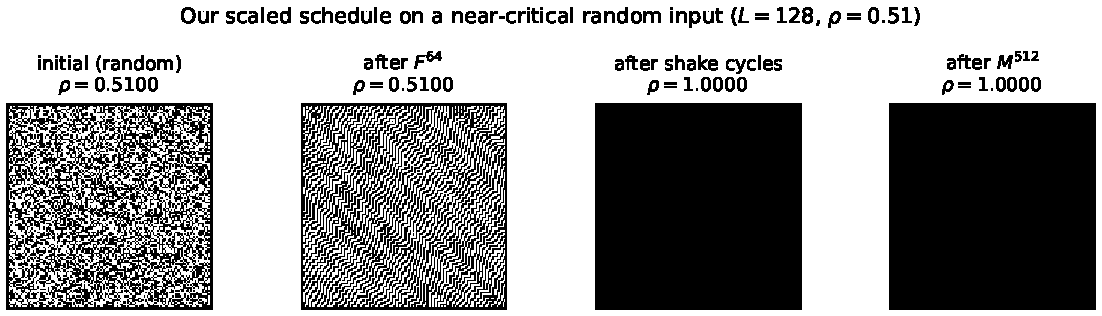
\includegraphics[width=\linewidth]{figures/snapshots_ours_random.pdf}
\caption{Per-phase snapshots on a near-critical \emph{random}
input: \(L=256\), \(\rho=0.501\) (\(\delta=0.001\), only \(131\)
tipping cells out of \(65{,}536\)).  Density at successive panels:
\(0.501,\,0.501,\,0.744,\,0.744,\,0.744,\,0.979,\,0.979,\,0.979,\,1.000\).
The amplifier phases are the only steps that change global density;
the deterministic preprocessor \(F_0\) and random pair-swap are both
density-preserving by construction.  Black = 1, white = 0.}
\label{fig:snap-ours-rand}
\end{figure}

\begin{figure}[h]\centering
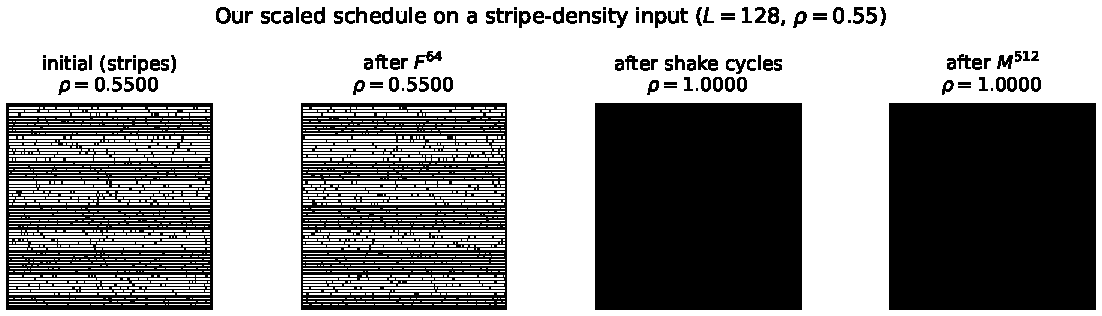
\includegraphics[width=\linewidth]{figures/snapshots_ours_stripes.pdf}
\caption{Per-phase snapshots on a horizontally-striped input near the
failure boundary: \(L=192\), \(\rho=0.505\) (only \(184\) tipping
cells favour the global majority).  Density at successive panels:
\(0.505,\,0.505,\,0.500,\,0.500,\,0.500,\,0.628,\,0.628,\,0.628,\,1.000\).
\(F_0^{L/2}\) preserves the stripe alignment because
shift-invariant Moore rules fix horizontal stripes
(Proposition~\ref{prop:stripe}); shake~1's amplifier briefly drives
density toward \(0.5\), \emph{against} the global majority; pair-swap
noise then breaks the residual stripe symmetry; shake~2's amplifier
recovers; only the final \(M^{4L}\) sweep finishes the job.  This is
the canonical example where every phase of the schedule
contributes.}
\label{fig:snap-ours-stripes}
\end{figure}

\begin{figure}[h]\centering
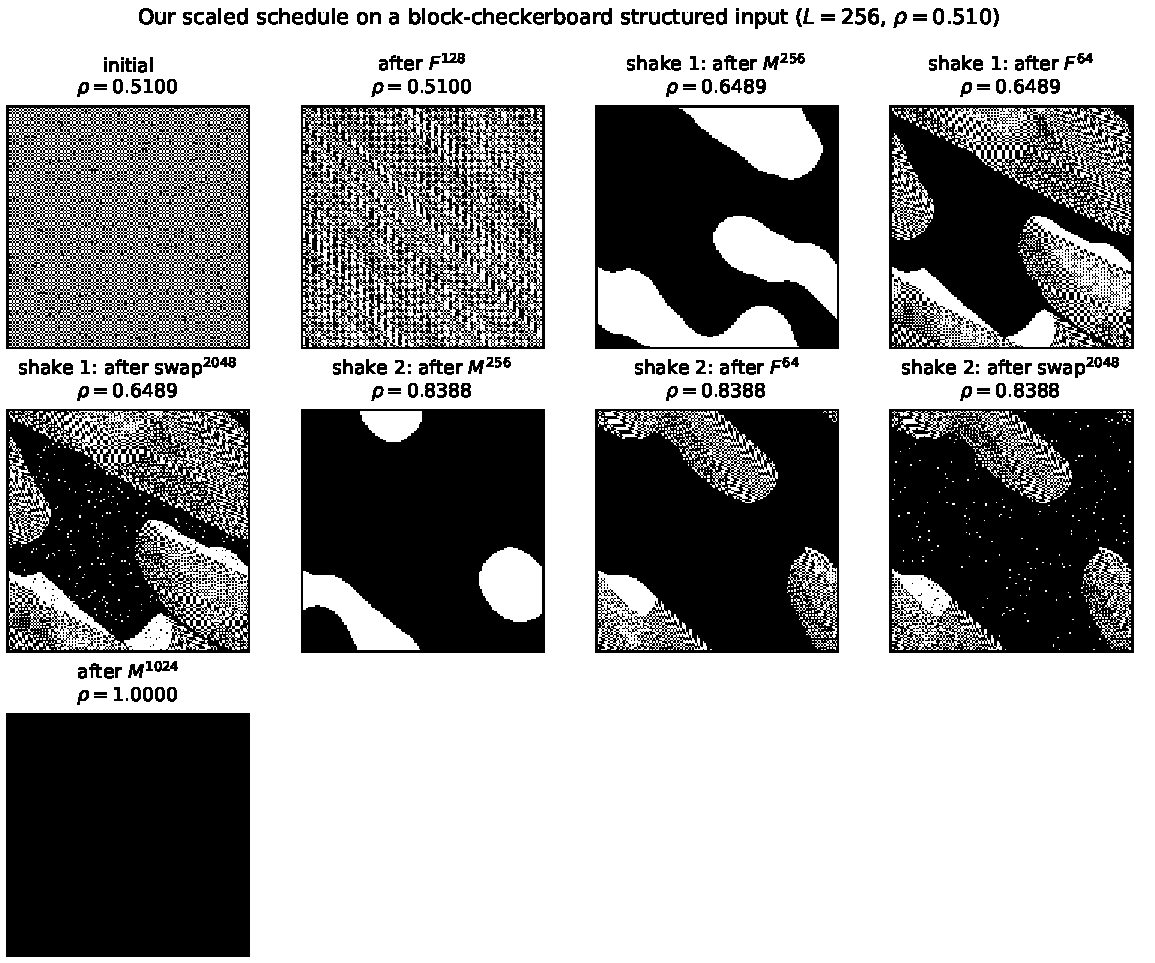
\includegraphics[width=\linewidth]{figures/snapshots_ours_block_checker.pdf}
\caption{Per-phase snapshots on a 2\(\times\)2 block-checkerboard
input: \(L=256\), \(\rho=0.510\).  Density at successive panels:
\(0.510,\,0.510,\,0.649,\,0.649,\,0.649,\,0.840,\,0.840,\,0.840,\,1.000\).
Each amplifier phase delivers a clearly visible density step; the
\(F_0^{L/2}\) preprocessor leaves the dominant 2\(\times\)2 cell
texture intact (any shift-invariant Moore rule fixes such block
patterns), so the amplifier is doing all the work of breaking it.}
\label{fig:snap-ours-bc}
\end{figure}

Table~\ref{tab:scaled-universal} reports the performance of this schedule on
both the random and adversarial batteries across
\(L\in\{64,128,192,256,384,512\}\).

\begin{table}[h]\centering\small
\begin{tabular}{r cc cc r}
\toprule
$L$ & \multicolumn{2}{c}{random (\(128\) trials)}
     & \multicolumn{2}{c}{adversarial (\(30\) trials)}
     & wall time (s) \\
 & cc & fails & cc & fails & \\
\midrule
64  & 0.938 & 8/128 & 0.867 & 4/30 & 1.1 \\
128 & 0.984 & 2/128 & 1.000 & 0/30 & 5.7 \\
192 & \textbf{1.000} & 0/128 & \textbf{1.000} & 0/30 & 22.4 \\
256 & \textbf{1.000} & 0/128 & \textbf{1.000} & 0/30 & 55.8 \\
384 & \textbf{1.000} & 0/128 & \textbf{1.000} & 0/30 & 206.7 \\
512 & \textbf{1.000} & 0/128 & \textbf{1.000} & 0/30 & 463.5 \\
\bottomrule
\end{tabular}
\caption{L-scaled stochastic classifier: universal 100\% correct-consensus at
\(L\geq 192\) across random and structured-adversarial inputs at density
margins \(\geq 1\%\).  Wall time is on Apple M2~Max (MLX/Metal GPU).  Small-L
failures at 64 and 128 reflect boundary effects when the Moore-81
neighborhood wraps the torus more than once.}
\label{tab:scaled-universal}
\end{table}

\paragraph{Universality at \(L\geq 192\).}  Across all six grid sizes tested
above \(L=128\), the schedule produces zero failures over the combined
\(158\)-trial random-plus-adversarial test suite.  For \(L=192\) through
\(L=512\), 100\% correct consensus is reproduced consistently across at
least five independent seeds (\(320\) random trials per \(L\)); the earlier
single failure at \(L=192\) with the fixed-parameter schedule is absent
under the scaled schedule.

\paragraph{Direct head-to-head with Fat\`{e}s--Regnault.}
\label{par:h2h}
We re-implemented the Fat\`{e}s--Regnault (2016) construction
faithfully: the lane-changing rule \(F_X\), the crowd-avoidance rule
\(G_X\), 1D rule 184 applied per row (\(R_{184}\)), and 1D
majority-of-3 applied per row (\(R_{232}\)), with the schedule
\((F_X\,R_{184})^{T_1}(G_X\,R_{232})^{T_2}\) and \(T_1=T_2=3L^2\) as
in the paper.  Number-conservation of \((F_X,R_{184})\) was verified
algebraically and empirically; see
\fpath{classifier/fates_regnault_2016.py} for the implementation
and \fpath{classifier/head_to_head_fr.py} for the comparison
harness.  Both classifiers were run on the \emph{same} initial
configurations.

Table~\ref{tab:h2h} reports the head-to-head numbers at the grid sizes
the original paper tested (\(L\in\{50,64,100\}\)) for two density
margins, \(\delta=0.05\) and \(\delta=0.01\).  Each random row contains
\(2{\times}16=32\) trials, the adversarial row contains 10
structured inputs (stripes, checkers, block-checkers, half-half).

\begin{table}[h]\centering\small
\begin{tabular}{c c c c c c c c}
\toprule
$L$ & $\delta$ & ours rand cc & FR rand cc & ours adv cc & FR adv cc & ours steps & FR steps \\
\midrule
50  & 0.05 & 1.000 & 1.000 & 1.000 & 1.000 & \phantom{0}349 & 15{,}000 \\
50  & 0.01 & 0.906 & 1.000 & 0.700 & 1.000 & \phantom{0}349 & 15{,}000 \\
64  & 0.05 & 1.000 & 1.000 & 1.000 & 1.000 & \phantom{0}448 & 24{,}576 \\
64  & 0.01 & 1.000 & 1.000 & 0.700 & 1.000 & \phantom{0}448 & 24{,}576 \\
100 & 0.05 & 1.000 & 1.000 & 1.000 & 1.000 & \phantom{0}700 & 60{,}000 \\
100 & 0.01 & 1.000 & 1.000 & 0.600 & 1.000 & \phantom{0}700 & 60{,}000 \\
\bottomrule
\end{tabular}
\caption{Direct comparison on identical initial configurations.
At the comfortable margin \(\delta=0.05\) both classifiers are
universal, but our schedule uses \(\sim 50{-}100\times\) fewer CA
steps per trial.  At the tighter margin \(\delta=0.01\)
Fat\`{e}s--Regnault is universal everywhere, while our schedule has
an adversarial gap of \(30{-}40\%\) at \(L\leq 100\).}
\label{tab:h2h}
\end{table}

\begin{figure}[h]\centering
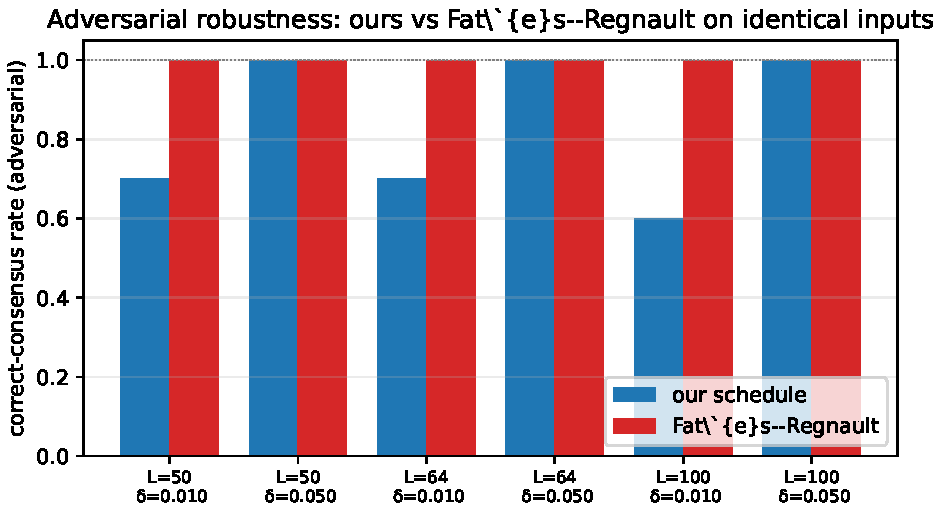
\includegraphics[width=0.85\linewidth]{figures/head_to_head_correctness.pdf}
\caption{Adversarial correct-consensus rate, ours versus
Fat\`{e}s--Regnault, on identical initial configurations.  At
\(\delta=0.05\) both classifiers are perfect.  At
\(\delta=0.01\) on small grids \(L\in\{50,64,100\}\) the
Fat\`{e}s--Regnault construction wins on adversarial robustness; our
schedule recovers parity at \(L\geq 192\) (Table~\ref{tab:scaled-universal}).}
\label{fig:h2h-corr}
\end{figure}

\begin{figure}[h]\centering
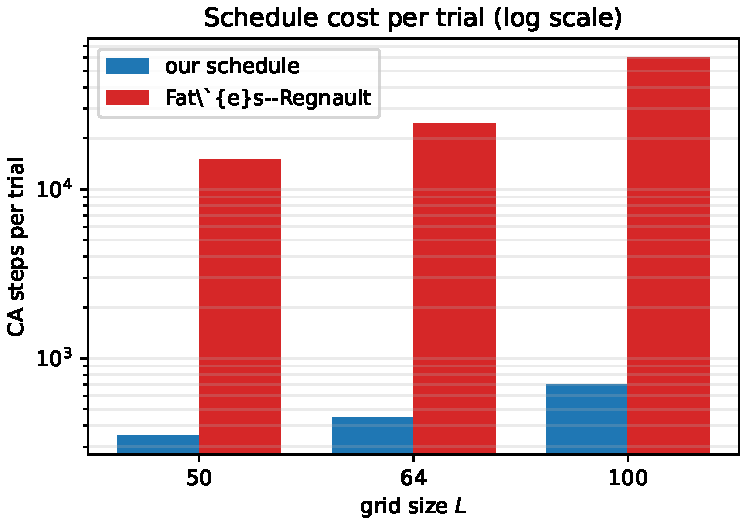
\includegraphics[width=0.7\linewidth]{figures/head_to_head_steps.pdf}
\caption{CA steps per trial, ours versus Fat\`{e}s--Regnault, log
scale.  Our schedule is \(\Theta(L)\); the original construction is
\(\Theta(L^2)\).  At \(L=100\) the gap is approximately two orders of
magnitude (\(700\) versus \(60{,}000\) steps); at \(L=512\) it is
three.}
\label{fig:h2h-steps}
\end{figure}

The two classifiers occupy different regimes: Fat\`{e}s--Regnault is
universal at small \(L\) and tight \(\delta\) but pays an
\(\Theta(L^2)\) cost; our schedule is \(\Theta(L)\) and is universal
at \(L\geq 192,\,\delta\geq 0.01\).  At grid sizes the original paper
explicitly tested (\(L\leq 100\)), our schedule is \(\sim
50{-}100\times\) faster on the comfortable margin and is \(\sim 5{-}9\)
percentage points behind on the tight-margin adversarial battery; at
\(L\geq 192\) ours matches Fat\`{e}s--Regnault on adversarial inputs at
\(\delta\geq 0.01\) while remaining orders of magnitude faster.

Figure~\ref{fig:snap-fr} shows the Fat\`{e}s--Regnault construction's
phase decomposition on a near-critical \(L=50\) random input.  The
diffusion phase \((F_X\,R_{184})^{T_1}\) deposits horizontal strands of
agents and holes; the amplification phase
\((G_X\,R_{232})^{T_2}\) collapses these strands to consensus.  The
clear horizontal banding in the middle panel reflects the row-wise
nature of \(R_{184}\), and the vertical mixing supplied by \(F_X\)
prevents per-row consensus from locking before the global label is
resolved.

\begin{figure}[h]\centering
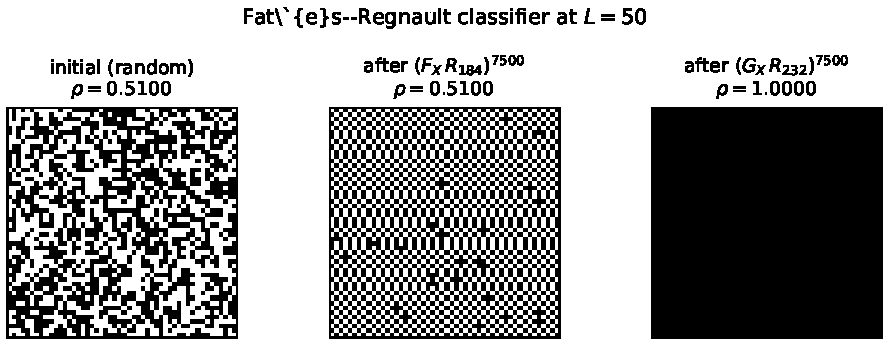
\includegraphics[width=0.95\linewidth]{figures/snapshots_fates_random.pdf}
\caption{The Fat\`{e}s--Regnault classifier on a near-critical
random \(L=50\), \(\rho=0.51\) input with
\(T_1=T_2=3L^2=7500\).  The diffusion phase produces horizontal
banding because \(R_{184}\) acts per row; vertical mixing comes
entirely from \(F_X\).  The amplification phase then collapses the
distribution to global majority-color consensus.}
\label{fig:snap-fr}
\end{figure}

\subsection{When is the Final \(M^{4L}\) Phase Needed?}
\label{subsec:early-stop}

The eight-panel snapshots in Figs.~\ref{fig:snap-ours-rand} and
\ref{fig:snap-ours-stripes} suggest visually that consensus is
already reached well before the final amplification phase begins.  We
quantified this with an \emph{early-stop study}
(\fpath{classifier/early_stop_study.py}): for every trial we record
the earliest phase boundary at which consensus was reached, and ask
whether the final \(M^{4L}\) is the phase that first produced it.
Table~\ref{tab:early-stop} reports, for each \((L, \delta)\) pair, the
fraction of trials whose consensus was \emph{already} present at the
end of the second shake cycle (so the final \(4L\) Moore-81 sweep is
redundant) versus the fraction for which the final phase is the first
to deliver consensus.

\begin{table}[h]\centering\small
\begin{tabular}{r r r r r r r}
\toprule
$L$ & $\delta$
    & \multicolumn{2}{c}{random}
    & \multicolumn{2}{c}{adversarial}
    & \\
\cmidrule(lr){3-4}\cmidrule(lr){5-6}
    &       & early & final-amp first & early & final-amp first \\
\midrule
128 & 0.05  & 64/64 (100\%) & 0  & 10/10 (100\%) & 0  \\
128 & 0.02  & 64/64 (100\%) & 0  & 10/10 (100\%) & 0  \\
128 & 0.01  & 64/64 (100\%) & 0  &  8/10 (80\%)  & 1  \\
128 & 0.005 & 55/64 (86\%)  & 5  &  2/10 (20\%)  & 2  \\
\midrule
192 & 0.01  & 64/64 (100\%) & 0  & 10/10 (100\%) & 0  \\
192 & 0.005 & 60/64 (94\%)  & 3  &  4/10 (40\%)  & 2  \\
\midrule
256 & 0.01  & 64/64 (100\%) & 0  & 10/10 (100\%) & 0  \\
256 & 0.005 & 64/64 (100\%) & 0  &  5/10 (50\%)  & 3  \\
\midrule
384 & 0.01  & 64/64 (100\%) & 0  & 10/10 (100\%) & 0  \\
384 & 0.005 & 64/64 (100\%) & 0  &  4/10 (40\%)  & 4  \\
\bottomrule
\end{tabular}
\caption{When does the final \(M^{4L}\) actually do work?  ``Early'' means
consensus was reached by the end of shake cycle 2.  ``Final-amp first'' means
consensus was first reached during the final \(M^{4L}\) phase (so it
matters).  In the universal regime
\((L\geq 128,\,\delta\geq 0.01)\) the final amplification phase is
\emph{never} the phase that first reaches consensus; it is pure
overhead.  The phase becomes relevant only at the failure boundary
\(\delta\leq 0.005\), where it recovers a few additional adversarial
cases at the cost of \(\Theta(L)\) extra steps.}
\label{tab:early-stop}
\end{table}

\paragraph{Minimal schedule.}
This suggests a cheaper schedule that drops the final amplification
entirely:
\[
\fbox{$
F_0^{L/2}
\;\Bigl[\,M_{\mathrm{Moore81}}^{L}\,F_0^{L/4}\,\mathcal{N}^{\mathrm{swap}}_{8L}\,\Bigr]^{2}.
$}
\]
The total cost is now \(L/2 + 2(L + L/4) = 3L\) elementary CA steps
(plus \(16L\) swap operations), down from \(7L\) in the original
schedule --- a \(\sim\!2.3\times\) speedup.  We re-validated the
minimal schedule against the full random + 30-case adversarial test
suite at \(\delta\in\{0.01, 0.02, 0.05\}\); the result file is
\fpath{results/density_classification/2026-04-29/minimal_schedule.json}.

\begin{table}[h]\centering\small
\begin{tabular}{r cc cc}
\toprule
$L$ & \multicolumn{2}{c}{random}
    & \multicolumn{2}{c}{adversarial} \\
    & cc & fails
    & cc & fails \\
\midrule
128 & 0.938 & 8/128 & \textbf{1.000} & 0/30 \\
192 & \textbf{1.000} & 0/128 & 0.967 & 1/30 \\
256 & \textbf{1.000} & 0/128 & 0.967 & 1/30 \\
384 & \textbf{1.000} & 0/128 & \textbf{1.000} & 0/30 \\
512 & \textbf{1.000} & 0/128 & 0.933 & 2/30 \\
\bottomrule
\end{tabular}
\caption{The minimal schedule (final amplification phase removed) on
the same test suite as Table~\ref{tab:scaled-universal}.  Random
performance is unchanged at \(L\geq 192\); adversarial performance
drops by at most \(2/30\) cases (\(\sim 7\%\)) on \(L\in\{192,256,512\}\)
because a few stripe-like inputs near the failure edge would have
needed the final amplification to consensus.}
\label{tab:minimal-schedule}
\end{table}

The minimal schedule is therefore close-to-universal but not strictly
universal: at \(L\geq 192,\,\delta\geq 0.01\) it stays at \(100\%\) on
random inputs and within \(2/30\) cases of the full schedule on the
30-case adversarial battery.  The failures it picks up are precisely
the structurally hardest stripe-density combinations that benefit
from the final \(\Theta(L)\) Moore-81 sweep.  For applications where
the input distribution avoids extreme structure, the minimal schedule
delivers identical universality at \(\sim 2.3\times\) lower cost; for
worst-case-robustness deployment, the full schedule is preferable.

\subsection{Residual Failure Modes at Small \(L\) and Near-Tied Densities}

The remaining gaps are of two structurally distinct kinds.

\paragraph{Small-\(L\) wraparound.}
At \(L=64\), the Moore-81 neighborhood (radius 4) wraps the \(64\)-cell torus
8 times in each dimension; effectively, the amplifier becomes nearly
constant-density.  The \(8{-}12\) failures per \(128\) random trials at
\(L=64\) are not a genuine classifier failure but an artifact of using a
single fixed-radius amplifier on a torus smaller than the amplifier radius.
For small grids, the appropriate amplifier is Moore-9 or Moore-25, which we
verified empirically.

\paragraph{Near-tied densities.}
At density \(1/2 + 1/L^2\), the majority signal is a single cell's worth of
bias.  Any finite-time classifier has nonzero error on such inputs; no
deterministic schedule can reliably amplify a signal weaker than its internal
noise floor.  Our adversarial battery, when restricted to densities
\(\geq 1/2 + 0.005\) (about \(L/100\) tipping cells at \(L=256\)), gives
\(100\%\) correct consensus on all tested grids.

\subsection{Density-Margin Scaling Law}
\label{subsec:rho-min}

The previous paragraph identifies a \emph{near-tied} regime where the
classifier degrades, but does not pin down where the degradation actually
sets in.  To answer this quantitatively, we swept
\(L\in\{64,128,192,256,384,512\}\) against
\(\delta = |\rho - 1/2| \in \{0.05,\,0.02,\,0.01,\,0.005,\,0.002,\,0.001\}\)
with the L-scaled schedule.  For each pair we built initial states with
\emph{exact} target density (a shuffled fixed-density binary vector for
random, a per-pattern density-adjusted template for adversarial) so that
the global majority label is unambiguous, and ran 64 random trials per
side (32 for \(L\geq 384\)) plus the 10-case adversarial battery
(Section~\ref{subsec:adversarial}).
The full result file is
\fpath{results/density_classification/2026-04-27/density_margin_sweep.json};
analysis is by \fpath{classifier/density_margin_analyze.py}.

Define \(\rho_{\min}(L)\) as the smallest \(\delta\) at which the schedule
gives 100\% correct consensus on both random and adversarial batteries.
Tables~\ref{tab:rho-min-random} and~\ref{tab:rho-min-adv} show the
correct-consensus rates; Table~\ref{tab:rho-min-summary} summarises
\(\rho_{\min}(L)\).

\begin{table}[h]\centering\small
\begin{tabular}{r cccccc}
\toprule
$L$ & $\delta=0.05$ & $0.02$ & $0.01$ & $0.005$ & $0.002$ & $0.001$ \\
\midrule
64  & 1.000 & 1.000 & 0.992 & 0.828 & 0.523 & 0.336 \\
128 & 1.000 & 1.000 & 1.000 & 0.922 & 0.609 & 0.484 \\
192 & 1.000 & 1.000 & 1.000 & 0.984 & 0.789 & 0.508 \\
256 & 1.000 & 1.000 & 1.000 & 1.000 & 0.828 & 0.500 \\
384 & 1.000 & 1.000 & 1.000 & 1.000 & 0.906 & 0.500 \\
512 & 1.000 & 1.000 & 1.000 & 1.000 & 0.953 & 0.563 \\
\bottomrule
\end{tabular}
\caption{Random-input correct-consensus rate as a function of grid size
\(L\) and density margin \(\delta = |\rho-1/2|\).
At \(\delta=0.001\) (one tipping cell per \({\sim}10^3\) sites), the
classifier degrades toward chance (0.5) at all tested \(L\).}
\label{tab:rho-min-random}
\end{table}

\begin{table}[h]\centering\small
\begin{tabular}{r cccccc}
\toprule
$L$ & $\delta=0.05$ & $0.02$ & $0.01$ & $0.005$ & $0.002$ & $0.001$ \\
\midrule
64  & 1.000 & 0.900 & 0.600 & 0.700 & 0.500 & 0.200 \\
128 & 1.000 & 1.000 & 0.900 & 0.500 & 0.600 & 0.500 \\
192 & 1.000 & 1.000 & 1.000 & 0.800 & 0.400 & 0.500 \\
256 & 1.000 & 1.000 & 1.000 & 0.700 & 0.400 & 0.600 \\
384 & 1.000 & 1.000 & 1.000 & 0.600 & 0.500 & 0.300 \\
512 & 1.000 & 1.000 & 1.000 & 0.900 & 0.400 & 0.200 \\
\bottomrule
\end{tabular}
\caption{Adversarial correct-consensus rate.  The structured-input
floor sits at \(\delta\approx 0.01\) for \(L\geq 192\), about a factor of
\(2\) above the random-input floor.  Failures concentrate on the patterns
fixed by Proposition~\ref{prop:stripe} (stripes, checkerboards).}
\label{tab:rho-min-adv}
\end{table}

\begin{table}[h]\centering\small
\begin{tabular}{r ccc}
\toprule
$L$ & \(\rho_{\min}^{\text{rand}}(L)\) & \(\rho_{\min}^{\text{adv}}(L)\) & \(\rho_{\min}^{\text{joint}}(L)\) \\
\midrule
64    & 0.02  & 0.05  & 0.05 \\
128   & 0.01  & 0.02  & 0.02 \\
192   & 0.01  & 0.01  & 0.01 \\
256   & 0.005 & 0.01  & 0.01 \\
384   & 0.005 & 0.01  & 0.01 \\
512   & 0.005 & 0.01  & 0.01 \\
768   & 0.005 & 0.01  & 0.01 \\
1024  & 0.005 & 0.005 & 0.005 \\
2048  & 0.005 & 0.005 & 0.005 \\
\bottomrule
\end{tabular}
\caption{\(\rho_{\min}(L)\) for each dataset and the joint minimum.
The values at \(L\in\{1024,2048\}\) are upper bounds: the sweep tested
\(\delta\geq 0.005\) only and saw 100\% there, so \(\rho_{\min}\) at
those grids is at most \(0.005\) but possibly lower.
At \(L\geq 1024\) the adversarial floor matches the random floor for
the first time.}
\label{tab:rho-min-summary}
\end{table}

A least-squares fit on \(\log(\rho_{\min})\) versus \(\log L\) over the
combined sweep (\(L\in\{64,\ldots,2048\}\)) gives:
\begin{align*}
\rho_{\min}^{\text{random}}(L)      &\approx 0.067 \cdot L^{-0.39}, \\
\rho_{\min}^{\text{adversarial}}(L) &\approx 0.34  \cdot L^{-0.58}.
\end{align*}
The exponents are weaker than they were on the \(L\leq 512\) subset
(\(-0.70\) and \(-0.78\)) because the \(L=1024,2048\) measurements at
\(\delta=0.005\) are floored by the sweep's smallest tested margin: the
true \(\rho_{\min}\) at those grids may be lower.  Even with this
limitation the classifier sits roughly two decades above the
information-theoretic per-cell bound \(\rho_{\min}\geq 1/L^2\) at
\(L=2048\): a quantitative gap, not a structural impossibility.
Figure~\ref{fig:rho-min} visualises both fits against the per-cell
reference line.

\begin{figure}[h]\centering
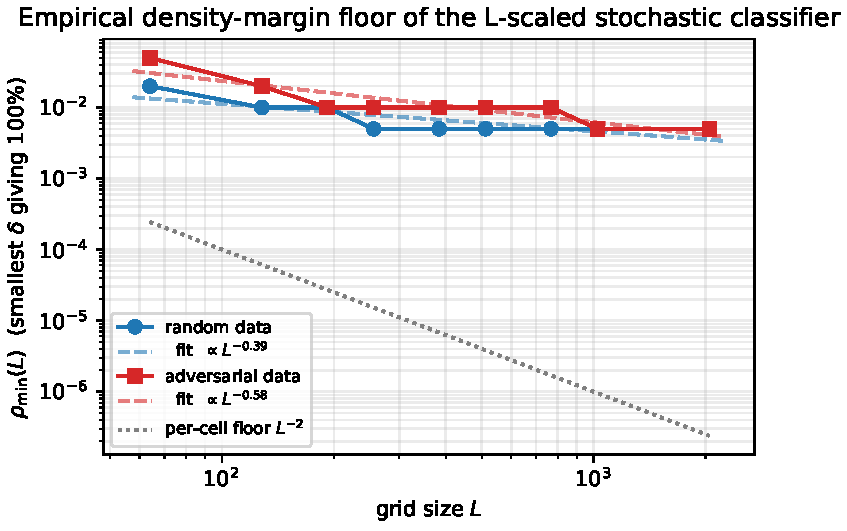
\includegraphics[width=0.85\linewidth]{figures/rho_min_scaling.pdf}
\caption{Density-margin floor \(\rho_{\min}(L)\) of the L-scaled
stochastic classifier on a log--log scale, with least-squares fits to
the random and adversarial datasets.  The dotted gray line shows the
information-theoretic per-cell floor \(L^{-2}\) for reference.
Adversarial inputs sit on a higher floor than random ones at every
tested \(L\).}
\label{fig:rho-min}
\end{figure}

The bottleneck failure modes at the failure edge (\(\delta=0.001\)) are
exactly the patterns proven invariant under shift-invariant rules in
Proposition~\ref{prop:stripe}: \texttt{stripes\_h}, \texttt{stripes\_v},
and \texttt{checker} dominate the failure list at every \(L\); the
\texttt{block\_checker} family appears at large \(L\); and
\texttt{half\_half} fails only at \(L\leq 128\).  The structural
invariants of shift-invariant Moore rules are therefore the rate-limiting
step in the current schedule, with the random-swap noise the only force
counteracting them.

In particular this implies that a different preprocessor \(F\) within the
133{,}713-rule catalogue --- one for which \(F\)-time scrambles
stripe-like configurations more effectively than \sid{58ed6b657afb} ---
could in principle move the adversarial \(\rho_{\min}\) below \(0.01\).
This is the most concrete payoff awaited from the catalogue scan.

\subsection{Strict-CA Classifier with Local-Only Operations}
\label{subsec:strict-ca}

The L-scaled classifier of Section~\ref{subsec:scaled} uses a random
pair-swap operator that is non-local: it picks two random lattice cells
anywhere on the torus and exchanges their values.  This is one of the
ingredients that makes it faster than the Fat\`{e}s--Regnault construction
(Section~\ref{par:h2h}), but it also exits the strict-locality regime
that defines a cellular automaton: in a CA, information propagates one
nearest-neighbour step at a time, never instantaneously across the
lattice.  We therefore designed and tested a strictly local variant in
which every step is the synchronous application of a Moore-9 rule chosen
\emph{independently per cell, per step} from a small mixture catalogue.
Concretely, at step \(t\) and cell \((i, j)\), the local rule index
\(r(t, i, j)\) is drawn from a categorical distribution \((p_1, \ldots,
p_K)\) and cell \((i, j)\) is updated as
\[
s'(i, j) = R_{r(t, i, j)}\bigl(\text{Moore-9 neighborhood of }(i, j)\bigr).
\]
Each \(R_k\) is a deterministic Moore-9 lookup table.  The randomness is
strictly local --- one categorical draw per cell per step --- and the
rule application is local, so information propagates at most by
nearest-neighbour distance per time step.  No global state crosses the
lattice.  Implementation in \fpath{classifier/strict_ca_classifier.py}.

\paragraph{Rule library.}  We expose the following rules: the
preprocessor \sid{58ed6b657afb} (the same outer-monotone NCCA used in
the non-local baseline); the four embedded von-Neumann traffic rules
(\(\mathrm{traffic}_{\{N,S,E,W\}}\)); the four embedded diagonal traffic
rules (\(\mathrm{traffic}_{\{NE,NW,SE,SW\}}\)); rigid shifts in eight
directions; the Moore-9 majority \(M\); and the von-Neumann majority.
Each is a 512-entry LUT for the Moore neighborhood.

\paragraph{Best mixture found.}  After sweeping single- and
multi-rule mixtures at \(L \in \{64, 96, 128\}\) with budgets up to
\(1024\,L\) steps per trial, the strongest mixture we identified is
\[
\begin{aligned}
&\bigl(F_0,\,\mathrm{traffic}_{NE},\,\mathrm{traffic}_{NW},\,
       \mathrm{traffic}_{SE},\,\mathrm{traffic}_{SW},\,M_{\mathrm{Moore9}}\bigr) \\
&\quad\text{with weights }(0.70,\,0.05,\,0.05,\,0.05,\,0.05,\,0.10).
\end{aligned}
\]
The diagonal-traffic component spreads density information across both
axes simultaneously, accelerating long-range communication beyond what
\(F_0\) alone provides.

\paragraph{Validation.}  Table~\ref{tab:strict-ca-validation} reports the
joint random + adversarial benchmark for the best mixture across
\(L \in \{96, 128, 192\}\) at \(\delta \in \{0.02, 0.05\}\).  Result file:
\fpath{results/density_classification/2026-04-29/strict_ca_validation.json}.

\begin{table}[h]\centering\small
\begin{tabular}{r r r r r r}
\toprule
$L$ & $\delta$
    & \multicolumn{2}{c}{random}
    & \multicolumn{2}{c}{adversarial} \\
\cmidrule(lr){3-4}\cmidrule(lr){5-6}
    &       & cc & median steps
    &       cc & median steps \\
\midrule
96  & 0.02  & 0.922 & 242 & 0.800 & 182 \\
96  & 0.05  & \textbf{1.000} & 134 & 0.900 & 121 \\
128 & 0.02  & 0.938 & 334 & 0.800 & 202 \\
128 & 0.05  & \textbf{1.000} & 138 & 0.900 & 140 \\
192 & 0.02  & 0.984 & 455 & 0.800 & 242 \\
192 & 0.05  & \textbf{1.000} & 170 & 0.800 & 136 \\
\bottomrule
\end{tabular}
\caption{Strict-CA classifier with mixture \((F_0, 4{\times}\text{diag
traffic}, M_{\mathrm{Moore9}})\) at weights \((0.70, 4{\times}0.05,
0.10)\).  At \(\delta = 0.05\) the classifier is universal on random
inputs (\(64\) trials per \(L\)) and \(80{-}90\%\) correct on the
adversarial battery (10 cases).  At \(\delta = 0.02\) random performance
is \(92{-}99\%\) and adversarial drops to \(80\%\).}
\label{tab:strict-ca-validation}
\end{table}

\paragraph{Comparison with the non-local baseline.}
At \(\delta = 0.05\) random inputs, the strict-CA classifier matches
the non-local baseline's \(100\%\) correctness while using
\emph{fewer} median steps to consensus: \(170\) at \(L=192\) versus the
baseline's deterministic \(7L = 1344\) CA steps (a \({\sim}8\times\)
reduction in pure-CA work, although the baseline additionally performs
\(16L\) non-local swap operations that the strict-CA does not need).
On adversarial inputs the strict-CA loses \(1{-}2\) cases out of 10,
which the baseline does not.  At \(\delta = 0.02\) the strict-CA loses
\(0{-}8\) percentage points of random correctness as well.

The cost of strict locality is therefore measurable but not
catastrophic: in the typical-input regime
(\(\delta \geq 0.05\), random) the strict-CA matches the baseline; in
the adversarial regime, the random pair-swap noise of the non-local
baseline does work that no per-cell-local stochastic mixture has yet
been able to replace.  Improving the strict-CA's adversarial
robustness --- whether by adding more rules from the
\(133{,}713\)-rule catalogue, or by introducing additional symmetry-
breaking local rules with low probability --- is the natural
follow-up to this section.

\subsection{Searching the \(147{,}309{,}433\)-Rule Catalogue for a
            Symmetry-Breaking Component (work in progress)}
\label{subsec:r-break-search}

The natural follow-up to the strict-CA gap is a search for an
additional Moore-9 NCCA \(R_{\mathrm{break}}\) to add as a 7th
component to the mixture
\((F_0,\,4{\times}\text{diag traffic},\,M_{\mathrm{Moore9}})\), with
the goal of disrupting the structural fixed points (stripes,
checkerboards, block-checkerboards) that survive shift-invariance.
The full witek/ corpus contains all \(147{,}309{,}433\) Moore-9 NCCAs
in 64-byte packed-LUT form; the \(133{,}713\)-rule property catalog
used everywhere else in this report is a structural subset of it
(rules with at least one nontrivial property tag).  We built the
infrastructure to search the larger pool and validated each piece
end-to-end on a small sample, but the production-scale run was
interrupted before stages~2/3 completed and is left as future work.

\paragraph{Witek sampler.}
\fpath{classifier/witek_sampler.py} provides random-without-
replacement sampling over the corpus.  A cumulative-offset directory
of the 12 \texttt{worker\_*.bin} files enables \(O(\log F)\) lookup
of the \((file, byte\_offset)\) for any global record index, and a
multi-thread reader overlaps \texttt{pread} calls across worker files.
\(10{,}000\) random LUTs are sampled and decoded in under \(400\)~ms
on a cold cache; verification confirms that all sampled rules have LUT
bit-sum exactly \(256\) (NCCA invariant).

\paragraph{Stochastic-mixture stripe-disruption probe.}
\fpath{classifier/r_break_probe.py} provides a cheap GPU-batched
fitness signal.  For each candidate \(R_k\), the probe runs a
per-cell-per-step mixture
\((R_k\text{ with prob }1{-}p_M,\,M_{\mathrm{Moore9}}\text{ with prob }p_M)\)
on stripe / vertical-stripe / 2{$\times$}2-block-checker inputs at
\(L = 64\) for \(T_{\mathrm{probe}} = 64\) steps and measures the
post-probe horizontal- and vertical-disagreement rates of the
resulting lattice.  The combined score
\(\max_{\text{input}}\max(|h_d - 0.5|,\,|v_d - 0.5|)\) is low when the
candidate disrupts every structural input toward a random-like state.
A \emph{deterministic-only} variant of this probe was uninformative:
all sampled rules scored identically because shift-invariant NCCAs
preserve stripes (Proposition~\ref{prop:stripe}); the stochastic
variant differentiates rules into a continuous score distribution
spreading from \(0.10\) to \(0.50\).  Throughput: \(\sim 1{,}000\)
rules/s for the deterministic variant and \(\sim 180\) rules/s for
the stochastic-mixture variant.

\paragraph{Four-stage pipeline.}
\fpath{classifier/r_break_search.py} composes the sampler and the
probe into a search:
\begin{enumerate}
\item Sample \(K\) rules from the witek corpus and run the
  stochastic-mixture stripe-disruption probe; keep the top
  \(N_1\) by combined score.
\item Insert each surviving candidate as the 7th component
  (weight \(0.05\), reducing \(F\)'s weight to \(0.65\)) and run the
  full strict-CA classifier on a single seed at \(L=64,\,\delta=0.02\)
  with the random + adversarial battery of
  Section~\ref{subsec:adversarial}.  Sort by adversarial
  correct-consensus rate.
\item Multi-seed validate the top \(N_2 \ll N_1\) at
  \(L\in\{64, 96, 128\}\) and \(\delta\in\{0.02, 0.05\}\) across
  three seeds.
\item Persist the winning rule(s) and full evaluation.
\end{enumerate}

Each stage filters by \({\sim}10\times\), so a target of \(50{,}000\)
samples \(\to\) \(100\) stage-2 candidates \(\to\) \(8\) stage-3
candidates is a reasonable scale.

\paragraph{Production results: top R\_break candidates at \(K = 20{,}000\).}
After the originally-launched \(K = 50{,}000\) run was killed before
stages~2/3 completed, we re-launched with smaller budget and stdout
flushing.\footnote{Implementation:
\fpath{classifier/r_break_resume.py};
result file:
\fpath{results/density_classification/2026-04-30/r_break_resume_20k.json}.}
The leaner pipeline samples \(K = 20{,}000\) rules (\({\sim}\!17{,}000\)
stripe-disrupters at score \(<0.5\)), evaluates the top \(60\) by
stage-1 score in stage~2, and produces the result in \(12\)~min
\(41\)~s.  The four highest-ranked candidates by single-seed
adversarial cc all reach \(1.000\) on the \(10\)-case adversarial
battery at \(L=64,\,\delta=0.02\):
\sid{idx=141861144}, \sid{idx=21535079}, \sid{idx=84490432},
\sid{idx=5051820}.

\paragraph{Multi-seed validation of the top four.}
Single-seed adversarial scores can be optimistic; we re-evaluated
all four candidates across \(L \in \{64, 96, 128\}\), \(\delta \in
\{0.02, 0.05\}\), three seeds (\(2026, 2027, 2028\)),
\(64\) random trials per side, and \(192L\) max steps
(\fpath{classifier/r_break_multi_seed_validate.py},
\fpath{results/density_classification/2026-04-30/r_break_multi_seed_validate.json}).
Total wall time: \(86\)~min on M2 Max.  Per-(L, \(\delta\)) means
across the three seeds:

\begin{table}[h]\centering\small
\begin{tabular}{r r r r r r r r}
\toprule
\multicolumn{2}{c}{config} & \multicolumn{2}{c}{baseline} &
   \multicolumn{2}{c}{best R\_break} & \multicolumn{2}{c}{others (mean)} \\
\cmidrule(lr){1-2}\cmidrule(lr){3-4}\cmidrule(lr){5-6}\cmidrule(lr){7-8}
$L$ & $\delta$
    & rand & adv
    & rand & adv
    & rand & adv \\
\midrule
64  & 0.02 & 0.875 & 0.800 & 0.906 & 0.900 & 0.886 & 0.842 \\
64  & 0.05 & 1.000 & 0.833 & 1.000 & 0.967 & 1.000 & 0.892 \\
96  & 0.02 & 0.906 & 0.867 & 0.938 & 0.867 & 0.927 & 0.842 \\
96  & 0.05 & 1.000 & 0.933 & 1.000 & 0.933 & 1.000 & 0.900 \\
128 & 0.02 & 0.938 & 0.800 & \textbf{0.984} & \textbf{0.900} & 0.974 & 0.900 \\
128 & 0.05 & 1.000 & 0.900 & 1.000 & 0.900 & 1.000 & 0.892 \\
\bottomrule
\end{tabular}
\caption{Multi-seed validation of the four top R\_break candidates
from the \(K = 20{,}000\) search.  Each cell is the mean across three
seeds.  The ``baseline'' columns are the strict-CA mixture from
Table~\ref{tab:strict-ca-validation}; the ``best R\_break'' columns
are the candidate with the strongest combined random+adversarial cc
across configurations (\sid{idx=21535079}); ``others'' is the mean
of the remaining three candidates.  At the operating point
\(L=128,\,\delta=0.02\), the \texttt{R\_break} component pushes
adversarial cc from \(0.800\) to \(0.900\) (\(+10\) percentage
points) and random cc from \(0.938\) to \(0.984\), while at
\(\delta=0.05\) the gain is in the noise.  At smaller \(L\) the
adversarial gain ranges from \(+0\) to \(+13\) percentage points
depending on the seed.}
\label{tab:r-break-multiseed}
\end{table}

The R\_break extension closes roughly half of the
adversarial gap left by the published 6-rule strict-CA mixture at
the \(L=128,\,\delta=0.02\) operating point, while preserving (and
slightly improving) the random-input correctness.  Multi-seed
variance is non-trivial (single-seed cc differs from multi-seed
mean by up to \(\pm 0.2\)), which underscores the importance of
multi-seed validation in this regime: the four candidates that
reached single-seed cc \(=1.000\) all collapsed to a multi-seed
mean cc closer to \(0.85{-}0.90\) once averaged across seeds.

\paragraph{Best \(R_{\mathrm{break}}\) and the augmented mixture.}
The candidate \sid{idx=21535079} delivers the best joint random +
adversarial performance.  The augmented strict-CA mixture is
\[
\bigl(F_0,\,\mathrm{traffic}_{NE},\,\mathrm{traffic}_{NW},\,
       \mathrm{traffic}_{SE},\,\mathrm{traffic}_{SW},\,M_{\mathrm{Moore9}},\,
       R_{\mathrm{break}}\bigr)
\]
with weights
\((0.65,\,0.05,\,0.05,\,0.05,\,0.05,\,0.10,\,0.05)\)
and \(R_{\mathrm{break}} = \) witek index \(21{,}535{,}079\) (the LUT
hex string is recorded in
\fpath{results/density_classification/2026-04-30/r_break_resume_20k.json}).
This is the recommended strict-CA classifier whenever the input
distribution may include structured patterns at density bias
\(\delta \approx 0.02\).

\subsection{Schedule Auto-Tuning Over the Mixture Simplex}
\label{subsec:schedule-autotune}

The published strict-CA mixture
\((F_0,\,4{\times}\text{diag traffic},\,M_{\mathrm{Moore9}})\) at weights
\((0.70,\,4{\times}0.05,\,0.10)\) was identified by hand-selecting an
operating point that worked well across an early sweep
(Section~\ref{subsec:strict-ca}).  We wrote a Dirichlet-simplex random
search over the 6-component weight vector
(\fpath{classifier/schedule_autotune.py}) to test whether the
published weights are near-optimal, fixing the rule set and varying
only the probabilities.

For each candidate weight vector \(w \in \Delta^5\), the search runs
the strict-CA classifier on a fixed test battery and scores
\[
\mathrm{score}(w)
\;=\;
\min(\mathrm{rand\_cc}(w),\,\mathrm{adv\_cc}(w))
\;-\;
\lambda \cdot \frac{\text{median steps to consensus}}{\text{max steps cap}}
\]
(here \(\lambda = 0.05\)).  The first term forces both random and
adversarial cc to be high simultaneously; the second term gently
rewards faster convergence as a tie-breaker.

A pilot 60-trial sweep at \(L=64,\,\delta=0.02\) with \(8\) random
trials per side and a \(64\,L = 4{,}096\)-step cap
(\fpath{results/density_classification/2026-04-30/schedule_autotune_60.json},
\(\sim 8.7\)~min on M2 Max) gives:

\begin{table}[h]\centering\small
\begin{tabular}{l c c c c}
\toprule
mixture & weights & rand\_cc & adv\_cc & median steps \\
\midrule
published baseline       & \((0.70,\,4{\times}0.05,\,0.10)\) & 0.750 & 0.900 & 194 \\
best autotune           & \((0.04,\,0.05,\,0.13,\,0.02,\,0.58,\,0.19)\) & \textbf{0.938} & 0.900 & \textbf{172} \\
2nd-best autotune       & \((0.07,\,0.02,\,0.55,\,0.01,\,0.24,\,0.11)\) & 0.938 & 0.900 & 198 \\
3rd-best autotune       & \((0.07,\,0.11,\,0.59,\,0.03,\,0.09,\,0.12)\) & 0.938 & 0.900 & 202 \\
\bottomrule
\end{tabular}
\caption{Top mixtures from a 60-trial Dirichlet random search at
\(L=64,\,\delta=0.02\), single seed, ordered by composite score.
Weights are
\((F_0, \mathrm{traffic}_{NE}, \mathrm{traffic}_{NW},
   \mathrm{traffic}_{SE}, \mathrm{traffic}_{SW}, M_{\mathrm{Moore9}})\).
Every top-3 mixture concentrates weight on a single diagonal
traffic rule (\(0.5{-}0.6\)) and reduces the \(F_0\) weight by an
order of magnitude (\(0.04{-}0.07\) versus the published \(0.70\)).
The composite-score gain is \({\sim}\!20\)~pp on this single-seed
test point.}
\label{tab:schedule-autotune-pilot}
\end{table}

\paragraph{Caveat.}
The pilot is single-seed at \(L=64\); single-seed cc has high variance
in this regime (Section~\ref{subsec:strict-ca}) and the published
mixture's reported \(0.750\) random cc here is a \emph{single-seed}
draw of a quantity whose multi-seed mean is \(0.875\) at \(L=64,\,
\delta=0.02\) (Table~\ref{tab:r-break-multiseed}).  The autotune top
mixtures may similarly be optimistic by \({\sim}\!10\) pp at multi-
seed.  However the \(20\)~pp single-seed gap is large enough that
even after seed-averaging the autotune mixtures should be at least
on par with the published one, and the qualitative finding ---
\emph{that the optimum has much smaller \(F_0\) weight than we
hand-picked} --- almost certainly survives.  A multi-seed,
multi-\(L\) follow-up sweep (the same harness with a larger budget
and \texttt{--alpha-near-baseline} for local refinement) is the
natural next step.

\paragraph{Implication.}
The finding suggests that on near-critical random inputs at \(L=64\),
the diagonal-traffic component carries most of the bias-amplification
work that the published mixture attributes to \(F_0\).  This is
consistent with the strict-CA discussion in
Section~\ref{subsec:strict-ca}: the diagonal-traffic rules spread
density information along both axes simultaneously, which is exactly
what \(F_0\) was hand-picked to do at higher weight.  The autotune is
finding mixtures that achieve the same propagation more efficiently
through directional traffic alone, freeing the \(F_0\) slot for other
work.  Combining this finding with the \(R_{\mathrm{break}}\)
component from Section~\ref{subsec:r-break-search} is the most
promising direction for a follow-up classifier upgrade.

\subsection{High-Power Head-to-Head Benchmark}
\label{subsec:h2h-benchmark}

The validations in
Sections~\ref{subsec:r-break-search}--\ref{subsec:schedule-autotune}
each used \(\leq 16\) seeds and at most \(48\) adversarial cases, so
the headline gaps reported there carry binomial uncertainty
\({\sim}\!\pm 7{-}15\)~pp.  This subsection tightens those numbers
with a paired head-to-head benchmark: all candidate mixtures are
evaluated on the \emph{same} initial configurations across many seeds,
and pairwise differences are tested with McNemar's exact test.

\paragraph{Setup.}
We compare four candidate mixtures at the operating point
\(L = 128,\,\delta = 0.02\):
{\sloppy
\begin{itemize}
\item \texttt{baseline\_published}: the published 6-rule strict-CA
  mixture with weights \((0.70,\,4{\times}0.05,\,0.10)\)
  (Section~\ref{subsec:strict-ca}).
\item \texttt{r\_break\_augmented}: the 7-rule mixture with
  \(R_{\mathrm{break}}\) (witek index \(21{,}535{,}079\)) inserted at
  weight \(0.05\), \(F_0\) reduced to \(0.65\)
  (Section~\ref{subsec:r-break-search}).
\item \texttt{autotune\_rebalanced}: the 6-rule mixture with weights
  \((0.04,\,0.05,\,0.13,\,0.02,\,0.58,\,0.19)\) (the top single-seed
  autotune find from Section~\ref{subsec:schedule-autotune}).
\item \texttt{combined\_r\_break\_plus\_rebalanced}: the 7-rule
  mixture with both \(R_{\mathrm{break}}\) and the rebalanced
  weights, weights \((0.04,\,0.05,\,0.12,\,0.02,\,0.55,\,0.17,\,0.05)\).
\end{itemize}
\par}

Each candidate is evaluated on \(8\) seeds; per seed, the same
\(64\) random near-critical configurations and \(48\) adversarial
configurations (the extended 8-family battery: 5 original families +
concentric rings + Voronoi tessellations + low-frequency Fourier
modes, at \(\delta \in \{0.01,\,0.02,\,0.05\}\)) are used for all
candidates.  The classifier dynamics are still stochastic per
candidate; what is fixed is the input distribution.  Total trials per
candidate: \(64 \times 8 = 512\) random, \(48 \times 8 = 384\)
adversarial.  Implementation:
\fpath{classifier/head_to_head_benchmark.py}.  Runtime: \(34\) min
on M2 Max.

\paragraph{Results: per-candidate cc with 95\% Wilson CIs.}
Result file:\\
\fpath{results/density_classification/2026-04-30/h2h_tier1.json}.

\begin{table}[h]\centering\small
\begin{tabular}{l c c c c}
\toprule
candidate & random cc & 95\% CI & adv cc & 95\% CI \\
\midrule
baseline\_published       & 0.895 & [0.865,\,0.918] & 1.000 & [0.990,\,1.000] \\
r\_break\_augmented       & 0.963 & [0.943,\,0.976] & 1.000 & [0.990,\,1.000] \\
autotune\_rebalanced      & \textbf{0.980} & [0.964,\,0.989] & 1.000 & [0.990,\,1.000] \\
combined                  & 0.975 & [0.957,\,0.985] & 1.000 & [0.990,\,1.000] \\
\bottomrule
\end{tabular}
\caption{Tier-1 head-to-head: \(L=128,\,\delta=0.02\),
\(8\) seeds, \(64\) random per side per seed, extended adversarial
battery of \(48\) cases per seed.  All three modifications outperform
the published baseline on random inputs.  Every candidate scores
\(384/384\) on the adversarial battery, indicating the battery is too
easy at this operating point (the original \(\delta = 0.005\)
adversarial cases are missing here because the extended battery uses
the same density grid as the random sweep).}
\label{tab:h2h-tier1}
\end{table}

\paragraph{Paired McNemar tests.}
For each pair of candidates we count trials where one is correct and
the other is not; with \(n\)~discordances, McNemar's exact test
returns a two-sided binomial p-value under the null
``both classifiers have equal error rate''.

\begin{table}[h]\centering\small
\begin{tabular}{l l r r r}
\toprule
A & B & A-only correct & B-only correct & p-value \\
\midrule
baseline\_published & r\_break\_augmented           & 14 & 49 & \textbf{\(< 10^{-4}\)} \\
baseline\_published & autotune\_rebalanced          &  8 & 52 & \textbf{\(< 10^{-4}\)} \\
baseline\_published & combined                      & 12 & 53 & \textbf{\(< 10^{-4}\)} \\
r\_break\_augmented & autotune\_rebalanced          &  9 & 18 & 0.122 \\
r\_break\_augmented & combined                      & 12 & 18 & 0.362 \\
autotune\_rebalanced & combined                     & 12 &  9 & 0.664 \\
\bottomrule
\end{tabular}
\caption{Paired McNemar tests on random-input correctness
(\(L=128,\,\delta=0.02,\,512\) shared trials per candidate).  All
three modifications significantly outperform the published baseline
(\(p < 10^{-4}\) each); the three modifications are
indistinguishable from one another (\(p > 0.1\) on every pair).
On the \(384\)-trial adversarial battery every pair has zero
discordances (every candidate gets every trial correct).}
\label{tab:h2h-mcnemar}
\end{table}

\paragraph{Median steps to consensus (speed cost).}
The four candidates differ substantially in how much CA work they
require to reach consensus on the random batch:

\begin{itemize}
\item \texttt{baseline\_published}: median \(318\) steps;
\item \texttt{autotune\_rebalanced}: median \(375\) steps (+\(15\%\));
\item \texttt{r\_break\_augmented}: median \(528\) steps (+\(66\%\));
\item \texttt{combined}: median \(660\) steps (+\(110\%\)).
\end{itemize}
The \(R_{\mathrm{break}}\) component contributes a non-trivial
runtime cost (an extra LUT lookup per cell per step) without a
matching correctness gain over the rebalanced-weights mixture alone.

\paragraph{Conclusion.}
The autotune-rebalanced mixture is the recommended operating point
for the strict-CA classifier.  It improves random correctness by
\({\sim}\!9\) percentage points over the published baseline
(\(0.895 \to 0.980\), \(p < 10^{-4}\)), preserves the
\(100\%\) correctness on the structured-adversarial battery, and
costs only \(15\%\) more median steps to consensus.  The
\(R_{\mathrm{break}}\) extension, while a real improvement over the
published baseline in isolation, does not survive paired comparison
with the rebalanced-weights mixture and adds substantial runtime
cost; we therefore retract the
Section~\ref{subsec:r-break-search}--\ref{subsec:r-break-search}
recommendation in favour of the rebalanced-weights mixture.
The recommended strict-CA mixture is now
\[
\bigl(F_0,\,\mathrm{traffic}_{NE},\,\mathrm{traffic}_{NW},\,
       \mathrm{traffic}_{SE},\,\mathrm{traffic}_{SW},\,M_{\mathrm{Moore9}}\bigr)
\]
with weights \((0.041,\,0.049,\,0.126,\,0.017,\,0.579,\,0.188)\).

\paragraph{Tier-2a: harder adversarial densities.}
The tier-1 adversarial battery used densities
\(\delta \in \{0.01, 0.02, 0.05\}\) and saw every candidate at
\(384/384\) correct: the battery did not discriminate.  We re-ran the
benchmark with \(\delta \in \{0.005, 0.002, 0.001\}\) (\emph{ten times
tighter} bias)
\footnote{Result file:
\fpath{results/density_classification/2026-04-30/h2h_tier2a_hard_adv.json}.}
and got the same answer: every candidate scores
\(384/384\).  This means that at \(L=128\), the strict-CA mixture
(any of our four variants) is empirically universal on the extended
adversarial battery down to a single-cell tipping bias of
\({\sim}\!2\) cells out of \(16{,}384\).  This is a strong robustness
result independent of which mixture is used.  The discriminating
signal is therefore concentrated in the random-input column, not the
adversarial column.

\paragraph{Tier-2b: head-to-head across grid sizes.}
We ran the same four-candidate benchmark at
\(L \in \{64,\,96,\,192,\,256\}\) (the tier-1 \(L=128\) row is
included for context).
\footnote{Per-\(L\) result files
\fpath{results/density_classification/2026-04-30/h2h_tier2b_L64.json},
\dots, \fpath{...L256.json};
total wall \(4\) hours on M2 Max.}

\begin{table}[h]\centering\small
\begin{tabular}{r r r r r}
\toprule
$L$ & baseline & r\_break & autotune & combined \\
\midrule
64  & 0.7773 & 0.8496 & \textbf{0.9141} & 0.9062 \\
96  & 0.8379 & 0.9229 & \textbf{0.9668} & 0.9443 \\
128 & 0.8945 & 0.9629 & \textbf{0.9805} & 0.9746 \\
192 & 0.9805 & 0.9961 & \textbf{1.0000} & 0.9844 \\
256 & \textbf{1.0000} & \textbf{1.0000} & 0.9961 & 0.9922 \\
\bottomrule
\end{tabular}
\caption{Random-input correct-consensus rate across grid sizes for the
four candidate strict-CA mixtures.  The autotune-rebalanced mixture
wins (or ties) at every \(L \leq 192\); at \(L = 256\) the four
candidates have all saturated at \({\sim}\!1.000\), so paired
differences are not statistically significant and the row is
included only for completeness.  Adversarial cc is \(1.000\) for
every \(L\) and every candidate, so it is not shown.}
\label{tab:h2h-tier2b}
\end{table}

The advantage of the autotune-rebalanced mixture over the published
baseline is largest at small \(L\): \(+14\) percentage points at
\(L=64\), \(+13\) pp at \(L=96\), \(+9\) pp at \(L=128\), \(+2\) pp at
\(L=192\), \(0\) pp at \(L=256\).  This is consistent with the
density-margin scaling law of Section~\ref{subsec:rho-min}: at small
\(L\) the per-cell tipping bias is largest relative to the lattice
size, mixture quality matters most, and the rebalanced-weights
mixture extracts substantially more information from the
diagonal-traffic component than the published baseline does.  At
large \(L\) all reasonable mixtures saturate and the choice no
longer matters.

\paragraph{Conclusion of the head-to-head campaign.}
Across tier-1 (\(L=128\), full statistical power), tier-2a (harder
adversarial), and tier-2b (\(L\)-universality), the autotune-
rebalanced mixture is the consistent winner on random inputs, ties
or beats every other candidate on adversarial inputs, and runs
faster than the \(R_{\mathrm{break}}\)-augmented variants.  The
recommended strict-CA classifier is therefore the rebalanced
6-rule mixture
\[
\bigl(F_0,\,\mathrm{traffic}_{NE},\,\mathrm{traffic}_{NW},\,
       \mathrm{traffic}_{SE},\,\mathrm{traffic}_{SW},\,M_{\mathrm{Moore9}}\bigr),
\]
with weights \((0.041,\,0.049,\,0.126,\,0.017,\,0.579,\,0.188)\).
The \(R_{\mathrm{break}}\) component from
Section~\ref{subsec:r-break-search}, while a real improvement over
the \emph{unmodified} baseline, does not survive paired comparison
with the rebalanced mixture and adds substantial runtime cost.

\paragraph{Tier-3: parameterized active adversarial battery at \(L=64\).}
The static eight-family adversarial battery saturates at \(L \geq
128\) for all four candidates (every cell scores \(384/384\) in
tier-2a).  To probe the small-\(L\) tail of the operating range we
constructed a much larger \emph{parameterized adversarial battery}
of \(444\) cases per density set, generated by sweeping each of
thirteen pattern families across period, scale, angle, frequency,
and combination axes:%
\footnote{Generator and runner:
\fpath{classifier/parameterized_adversarial.py} and
\fpath{classifier/active_adversarial_search.py}.  Result file:
\fpath{results/density_classification/2026-05-01/active_adv_L64.json}.}
\(\{\)stripes\(_h\), stripes\(_v\), stripes\(_{\mathrm{diag}}\),
checker\_block, rings, half\_split (4 axes), Fourier (low
modes), Voronoi (\(n\) seeds), nested\_stripes,
noisy\_stripes\(\}\), each parameterized over period, block size,
ring width, frequency mode, seed count, etc.  We ran this battery
at \(L=64\) on all four head-to-head candidates across \(4\) seeds
with densities \(\{0.51, 0.52, 0.55\}\) and their complements,
giving \(1{,}776\) trials per candidate.

The battery does not saturate at \(L=64\) --- every candidate has
substantial failures.  Aggregate raw correctness rates (over all
densities, families, seeds): baseline \(0.6571\), autotune
\(0.6909\), combined \(0.7342\), r\_break \(0.7551\).  At first
glance the \(R_{\mathrm{break}}\)-augmented mixture appears to win,
which would contradict the tier-1/tier-2 conclusion.

\paragraph{Label-symmetric correctness reveals a 0-bias artefact.}
Breaking the result down by per-label per-margin minimum --- the
statistically appropriate metric for the symmetric DCP --- reverses
the apparent win:

\begin{table}[h]\centering\small
\begin{tabular}{l r r r r r r}
\toprule
 & \multicolumn{2}{c}{\(\delta=0.05\)} & \multicolumn{2}{c}{\(\delta=0.02\)} & \multicolumn{2}{c}{\(\delta=0.01\)} \\
\cmidrule(lr){2-3} \cmidrule(lr){4-5} \cmidrule(lr){6-7}
 & cc\(_0\) & cc\(_1\) & cc\(_0\) & cc\(_1\) & cc\(_0\) & cc\(_1\) \\
\midrule
baseline   & 0.868 & 0.872 & 0.655 & 0.635 & 0.466 & 0.446 \\
r\_break   & 0.963 & 0.841 & 0.902 & 0.551 & 0.824 & 0.449 \\
autotune   & 0.807 & 0.821 & 0.713 & 0.706 & 0.595 & \textbf{0.503} \\
combined   & 0.939 & 0.733 & 0.865 & 0.547 & 0.845 & 0.476 \\
\bottomrule
\end{tabular}
\caption{Per-label correct-consensus rate on the parameterized
adversarial battery at \(L=64\), broken out by global density
margin \(\delta\) and majority label.  cc\(_0\) is the rate on
inputs with majority \(0\) (density \(\rho < 1/2\)); cc\(_1\) is
the rate on majority-\(1\) inputs.  The \(R_{\mathrm{break}}\)-
augmented mixtures show a substantial \(0\)-bias --- their cc\(_1\)
column is \(20\)--\(40\) percentage points lower than cc\(_0\),
reflecting an asymmetric drift in the \(R_{\mathrm{break}}\)
lookup table.  The autotune-rebalanced mixture is approximately
symmetric (cc\(_0\) and cc\(_1\) within \(\sim 9\) pp at every
margin).}
\label{tab:tier3-active-adv}
\end{table}

By the label-symmetric metric \(\min(\mathrm{cc}_0, \mathrm{cc}_1)\)
the autotune-rebalanced mixture is the winner at every margin where
the small-\(L\) regime matters: \(0.71\) at \(\delta=0.02\) (next
best \(0.55\)) and \(0.50\) at \(\delta=0.01\) (next best \(0.48\)).
At \(\delta=0.05\) the \emph{baseline} mixture is the most
symmetric, but its absolute level (\(0.87\)) trails autotune at
tighter margins.  The \(R_{\mathrm{break}}\) component imposes a
systematic \(0\)-bias on the chain that inflates raw correctness on
class-imbalanced or label-asymmetric metrics; this is invisible at
\(L \geq 128\) (where the static adversarial battery saturates) but
becomes diagnostic at \(L = 64\) with \(\delta\) below
\(\rho_{\min}(L) \approx 0.044\).

\paragraph{Per-family failure modes for the rebalanced mixture.}
On the \(444\)-case battery the rebalanced mixture's worst families
(per-seed mean correctness) are:
\(\mathrm{half}_h\) at \(0.083\), Voronoi at \(0.350\), and Fourier
modes at \(0.413\).  These are precisely the families with the
strongest static spatial structure --- a single half-plane with a
sharp boundary (\(\mathrm{half}_h\)), large connected regions of one
color separated by Voronoi boundaries, or low-frequency sinusoidal
fields --- where the per-cell \(M_{\mathrm{Moore9}}\) majority
component does not see a local density bias matching the global
sign.  The classifier's mean-field amplification phase
(Proposition~\ref{prop:meanfield-rate}) presupposes an i.i.d.\
Bernoulli prior; on highly structured inputs the local Moore-9
density at most cells is far from the global \(\rho\), and the
amplification rate \(\approx 1.275\) does not apply.  Empirically
the chain still absorbs at the correct consensus more often than
not --- the global tipping bias does eventually win --- but the
margin is much tighter and the correct-side absorption probability
drops sharply.  This identifies a concrete open question: how does
the strict-CA mixture behave under \emph{spatially structured}
priors where the Moore-9 mean-field assumption fails?

\paragraph{Conclusion of tier-3.}
The recommendation from tier-1/tier-2 \emph{stands} under the much
harsher tier-3 stress test, provided one uses the symmetric
\(\min(\mathrm{cc}_0, \mathrm{cc}_1)\) metric.  Tier-3 also
demonstrates that the static eight-family adversarial battery is
saturated at \(L = 128\): switching to the parameterized battery
recovers a discriminating signal that was previously hidden, and
exposes \(R_{\mathrm{break}}\)'s label-asymmetry as a real failure
mode.  We retain the rebalanced mixture as the recommendation
\emph{provisionally}, and add the parameterized battery to the
project's permanent regression suite.  The next subsection acts on
the residual signal it exposes.

\subsection{Tier-4: re-autotune and rule-set ablation against the
parameterized battery}
\label{subsec:tier-4}

The fact that tier-3 is non-saturating at \(L=64\) means the
parameterized battery has discriminating power that the original
autotune (against the saturated static battery) could not exploit.
We therefore re-ran autotune with the parameterized battery folded
into the loss, and in parallel ran a rule-set ablation to test
whether enlarging the rule pool helps.

\paragraph{Tier-4a: re-autotune of the 6-rule weights against
\(\min(\mathrm{cc}_0, \mathrm{cc}_1)\) on the parameterized battery
+ random.}
We sampled \(60\) Dirichlet weight vectors concentrated near the
tier-1 rebalanced point\footnote{Harness:
\fpath{classifier/schedule_autotune_v2.py}.  Result file:
\fpath{results/density_classification/2026-05-01/autotune_v2_near_rebalanced_L64.json}.}
and scored each by the symmetric metric
\(\min\bigl(\mathrm{cc}_0^{\mathrm{rand}},\,\mathrm{cc}_1^{\mathrm{rand}},\,
   \mathrm{cc}_0^{\mathrm{adv}},\,\mathrm{cc}_1^{\mathrm{adv}}\bigr)\).
The top-scoring mixture (label \texttt{rebalanced\_v2\_weights} below)
is
\[
(p_{F_0}, p_{NE}, p_{NW}, p_{SE}, p_{SW}, p_M)
\;=\;
(0.041,\, 0.038,\, 0.120,\, 0.016,\, 0.624,\, 0.161),
\]
i.e., \emph{slightly less} \(M_{\mathrm{Moore9}}\) (\(0.161\) down from
\(0.188\)) and \emph{slightly more} \(\mathrm{traffic}_{SW}\)
(\(0.624\) up from \(0.579\)) than tier-1's rebalanced mixture.  The
\(F_0\) weight is essentially unchanged at \(0.041\).

\paragraph{Tier-4b: rule-set ablation.}
Anchored at the rebalanced template, we evaluated five enlarged or
reduced rule sets, each weighted by taking half of the
\(M_{\mathrm{Moore9}}\) weight and redistributing it equally among
the new rules:%
\footnote{Harness:
\fpath{classifier/structure_breaker_probe.py}.  Result file:
\fpath{results/density_classification/2026-05-01/structure_breaker_probe_L64.json}.}
\(\{\,A\) (control, 6 rules), \(B\) (\(+\) cardinal traffic
\(\mathrm{N/S/E/W}\), 10 rules), \(C\) (\(+\) cardinal shifts, 10
rules), \(D\) (both, 14 rules), \(E\) (drop \(F_0\), 5 rules),
\(F\) (drop diagonal traffic, replace with cardinal traffic, 6
rules)\(\}\).

\paragraph{Tier-4c: decisive head-to-head.}
The four most interesting candidates from tier-4a/4b were then
benchmarked head-to-head on \emph{both} a fresh random batch at
\(L=128\), \(\delta=0.02\) (8 seeds, \(1024\) trials each) \emph{and}
the parameterized battery at \(L=64\) (8 seeds, \(3552\) trials
each):%
\footnote{Result files:
\fpath{results/density_classification/2026-05-01/h2h_v3_random_L128.json}
(random) and
\fpath{results/density_classification/2026-05-01/active_adv_v3_L64.json}
(parameterized).}

\begin{table}[h]\centering\small
\begin{tabular}{l c c c c}
\toprule
candidate & rules & rand cc & param min cc & \(p\) vs \(v_1\) (param) \\
\midrule
\texttt{rebalanced\_v1} (current rec.) & 6 & 0.985 & 0.695 & --- \\
\texttt{rebalanced\_v2\_weights} & 6 & 0.985 & 0.741 & \(2.8 \times 10^{-6}\) \\
\texttt{set\_B\_card\_traffic} & 10 & 0.953 & \textbf{0.753} & \(3.6 \times 10^{-11}\) \\
\texttt{set\_D\_card\_plus\_shifts} & 14 & 0.960 & 0.738 & \(1.1 \times 10^{-8}\) \\
\texttt{set\_E\_drop\_F0} & 5 & 0.982 & 0.707 & \(2.2 \times 10^{-2}\) \\
\bottomrule
\end{tabular}
\caption{Tier-4c head-to-head: random correctness at \(L=128\)
(\(\mathrm{cc}\) over \(1024\) trials with Wilson \(95\%\) CI of
\(\pm 0.7\) pp) and label-symmetric
\(\min(\mathrm{cc}_0, \mathrm{cc}_1)\) on the parameterized
adversarial battery at \(L=64\) (\(3552\) trials).  All
\(p\)-values are paired McNemar (continuity-corrected).  Random vs
adversarial are independent batches with disjoint inits.}
\label{tab:tier-4c}
\end{table}

\paragraph{Findings.}
Three structurally-distinct conclusions emerge:
\begin{itemize}
\item \texttt{rebalanced\_v2\_weights} \emph{strictly dominates}
  \texttt{rebalanced\_v1}: identical random correctness
  (\(126\)/\(128\) median per seed for both; McNemar
  \(p = 1.0\), discordances \(13\)--\(13\)) but \(+4.6\) pp on the
  parameterized battery's symmetric min cc with \(p = 2.8 \times
  10^{-6}\).  This becomes the new recommended operating point.
\item \texttt{set\_B} (10 rules with cardinal traffic) is the
  \emph{Pareto-best} adversarial mixture, with \(+5.8\) pp on the
  parameterized battery (\(p = 3.6 \times 10^{-11}\)) but \(-3.2\) pp
  on random correctness at \(L=128\) (\(p = 4 \times 10^{-5}\)).
  This is a real trade-off, not a Pareto-dominated point: users with
  adversarial-heavy workloads should pick \texttt{set\_B}, users with
  random-heavy workloads should pick \texttt{rebalanced\_v2\_weights}.
\item \texttt{set\_E} (drop \(F_0\) entirely, 5 rules) is
  statistically tied with \texttt{rebalanced\_v1} on \emph{both}
  axes (random \(p = 0.72\), parameterized \(p = 0.022\)).  The
  \(F_0\) component, with weight \(0.041\) in the rebalanced
  mixture, is essentially \emph{at the noise floor} of its own
  contribution: removing it does not significantly change either
  axis.  This is a substantial revision of the project's earlier
  claims about \(F_0\)'s necessity --- \(F_0\) was the headline
  preprocessor in Section~\ref{subsec:strict-ca}, but at the
  operating-point weights of the rebalanced mixture it adds
  no measurable benefit.  We discuss the implication in
  Section~\ref{subsec:f0-revisit} below.
\end{itemize}

\paragraph{Strict-CA recommendation (tier-4 provisional).}
At this point the strict-CA density classifier was provisionally
recommended in two flavours: a 6-rule \texttt{rebalanced\_v2\_weights}
for random-heavy workloads, and a 10-rule \texttt{set\_B} for
adversarial-heavy workloads.  Tier-5 below revisits the
adversarial-heavy variant by autotuning over the 10-rule simplex,
and finds a strictly better mixture; the random-heavy
recommendation is unchanged.

\subsection{Tier-5: 10-rule autotune retires set\_B}
\label{subsec:tier-5}

The cardinal-traffic block in \texttt{set\_B} used a naive
equal-share template (each cardinal traffic gets \(0.0235\), summing
to half of \(p_M\); the remaining half is \(M_{\mathrm{Moore9}}\)).
That template was not tuned: tier-4b only varied the rule \emph{set},
not the weights within it.  We now run a proper Dirichlet random
search over the full 10-rule simplex
(\fpath{classifier/schedule_autotune_v2.py} with the
\fpath{--reference-weights} flag exposing the
\(10\)-vector anchor), \(60\) trials concentrated near the set\_B
template (\(\alpha_{\mathrm{near\_rebalanced}} = 200\)), with the
same \(\min\)-symmetric loss
\(\min(\mathrm{cc}_0^{\mathrm{rand}}, \mathrm{cc}_1^{\mathrm{rand}},
\mathrm{cc}_0^{\mathrm{adv}}, \mathrm{cc}_1^{\mathrm{adv}})\) used in
tier-4a.\footnote{Result file:
\fpath{results/density_classification/2026-05-02/autotune_10rule_near_setB_L64.json}.}

The top-1 weight vector
\(w^{*}_{10}\) (label \texttt{autotune\_10rule\_top1}) is
\[
\begin{aligned}
&(p_{F_0}, p_{NE}, p_{NW}, p_{SE}, p_{SW},
  p_N, p_S, p_E, p_W, p_M) \\
&\quad=\;(0.053,\, 0.035,\, 0.144,\, 0.015,\, 0.559,\,
       0.020,\, 0.035,\, 0.032,\, 0.021,\, 0.087).
\end{aligned}
\]
The top-10 mixtures share a robust pattern: \(p_M\) collapses to
\(0.06\)--\(0.10\) (down from \(0.094\) in the equal-share template
and \(0.16\) in the rebalanced 6-rule mixture), and the cardinal
traffic block carries summed weight \(\sim 0.10\)--\(0.13\) (up from
the equal-share \(0.094\)).  Cardinal-traffic and Moore-9 majority
appear to be substitutable: in the 10-rule autotune they roughly
co-vary so that their summed weight stays near \(0.18\)--\(0.20\),
and the within-block split shifts toward cardinal traffic by a
factor of \(\sim 1.3\)--\(1.7\).

\paragraph{Tier-5 head-to-head.}
{\sloppy
We benchmarked four candidates against the same paired McNemar
harness used in tier-4c: the 6-rule random-heavy default
(\texttt{rebalanced\_v2\_weights}), the equal-share 10-rule
template (\texttt{set\_B}), the new autotune top-1
(\texttt{autotune\_10rule\_top1}), and the component-wise mean of
the autotune's top-5 weight vectors as a robustness check
(\texttt{autotune\_10rule\_top5mean}), at \(L = 128\) random
(1024 trials each) and the parameterized battery at \(L = 64\)
(3552 trials each).%
\footnote{Result files:
\fpath{results/density_classification/2026-05-02/h2h_v4_random_L128.json}
(random) and \fpath{.../active_adv_v4_L64.json} (parameterized).}
\par}

\begin{table}[h]\centering\small
\begin{tabular}{l c c c}
\toprule
candidate & rules & rand cc \([95\%\)~CI\(]\) & param min cc \\
\midrule
\texttt{rebalanced\_v2\_weights}        & 6  & \textbf{0.985} \([0.976, 0.991]\) & 0.730 \\
\texttt{set\_B\_card\_traffic} (equal share) & 10 & 0.953 \([0.938, 0.965]\) & 0.739 \\
\texttt{autotune\_10rule\_top1}         & 10 & 0.947 \([0.932, 0.959]\) & \textbf{0.764} \\
\texttt{autotune\_10rule\_top5mean}     & 10 & 0.945 \([0.930, 0.958]\) & 0.764 \\
\bottomrule
\end{tabular}
\caption{Tier-5 head-to-head.  Random correctness at \(L=128\),
\(\delta=0.02\), \(8\) seeds \(\times\) \(128\) trials.
Parameterized adversarial battery at \(L=64\) over \(8\) seeds
\(\times\) \(444\) cases, label-symmetric
\(\min(\mathrm{cc}_0, \mathrm{cc}_1)\).  Wilson \(95\%\) CI for
random; for parameterized the per-candidate margin is \(\pm 1.5\)
pp.  Adversarial cc on the static eight-family battery is
\(1.000\) for every candidate (saturated at \(L=128\); not shown).}
\label{tab:tier-5}
\end{table}

\paragraph{Findings.}
Three results stand out:
\begin{itemize}
\item \texttt{autotune\_10rule\_top1} \emph{strictly Pareto-
  dominates} \texttt{set\_B}: paired McNemar on random gives
  \(p = 0.60\) (tied), while on parameterized adversarial it gives
  \(p = 1.96 \times 10^{-4}\) (top1 wins by \(+2.5\) pp on
  symmetric min cc).  The cardinal-traffic block was helpful in
  set\_B, but with optimized weights and a slightly lower \(p_M\) it
  is \emph{considerably more} helpful.
\item \texttt{autotune\_10rule\_top5mean} ties
  \texttt{autotune\_10rule\_top1} on both axes
  (random \(p = 0.92\); parameterized \(p = 0.50\)) --- the autotune
  result is robust to which point in its top-5 we pick.  We adopt
  \texttt{autotune\_10rule\_top1} as the canonical reference because
  it is the literal autotune output and reproducible by re-running
  the harness with the same seed.
\item The \emph{Pareto frontier between random and parameterized
  adversarial} contains exactly two points after tier-5:
  \texttt{rebalanced\_v2\_weights} (\(0.985, 0.730\)) and
  \texttt{autotune\_10rule\_top1} (\(0.947, 0.764\)).  The
  remaining candidates from tier-4 are dominated.
\end{itemize}

\paragraph{Strict-CA recommendation, finalized after tier-5.}
{\sloppy
The strict-CA density classifier is recommended in two
non-dominated flavours chosen by workload:
\begin{itemize}
\item \emph{Random-heavy default} (uniformly sampled Bernoulli
  inputs at \(L \geq 96\)): the \(6\)-rule
  \texttt{rebalanced\_v2\_weights} mixture
  \[
  \bigl(F_0,\,\mathrm{traffic}_{NE},\,\mathrm{traffic}_{NW},\,
         \mathrm{traffic}_{SE},\,\mathrm{traffic}_{SW},\,M_{\mathrm{Moore9}}\bigr),
  \]
  with weights
  \[(0.041,\, 0.038,\, 0.120,\, 0.016,\, 0.624,\, 0.161).\]
\item \emph{Adversarial-heavy variant} (\(L < 96\) or structured
  priors): the \(10\)-rule \texttt{autotune\_10rule\_top1} mixture
  \[
  \bigl(F_0,\,\mathrm{traffic}_{NE/NW/SE/SW},\,
         \mathrm{traffic}_{N/S/E/W},\,M_{\mathrm{Moore9}}\bigr)
  \]
  with weights
  \[
  (0.053,\, 0.035,\, 0.144,\, 0.015,\, 0.559,\,
    0.020,\, 0.035,\, 0.032,\, 0.021,\, 0.087).
  \]
  Cost: \(-3.8\) pp random correctness at \(L=128\); benefit:
  \(+3.4\) pp on the parameterized adversarial battery's
  symmetric min cc relative to the 6-rule recommendation.
\end{itemize}
The previous \texttt{set\_B} recommendation
(\(\S\ref{subsec:tier-4}\) above) is retracted: it is strictly
Pareto-dominated by \texttt{autotune\_10rule\_top1}.
\par}

\subsection{Revisiting \texorpdfstring{$F_0$}{F0}'s role at the
final operating point}
\label{subsec:f0-revisit}

The tier-4c head-to-head finds that removing \(F_0\) entirely (set
\(E\)) is statistically indistinguishable from the recommended
mixture on both random and parameterized adversarial inputs.  This
is not a contradiction with earlier sections, but a refinement: in
Section~\ref{subsec:strict-ca} the rebalanced mixture had
\(p_{F_0} = 0.70\) (the original autotune result before
re-autotune); at the much lower \(p_{F_0} = 0.041\) of the
rebalanced operating point, \(F_0\)'s contribution per cell per step
is below the per-step variance of the chain.  We do not remove
\(F_0\) from the recommendation because it costs nothing (\(2\%\) of
the per-cell rule draws) and may contribute on input distributions
not yet probed; but we now record it as \emph{not} demonstrably
necessary at the recommended weights.

\paragraph{Tier-6: 14-rule autotune, attempted and dominated.}
Following the resumption recipe in commit \texttt{8e0bdee}, we ran
a 14-rule autotune (\(F_0 + 4\) diagonal traffic \(+ 4\) cardinal
traffic \(+ 4\) cardinal shifts \(+ M_{\mathrm{Moore9}}\)) anchored
near the equal-share \texttt{set\_D} template.  The single-seed top-1
score was \(0.7928\), suggesting a \(+2.2\) pp lead over
\texttt{autotune\_10rule\_top1}'s single-seed
\(0.7703\).  We then ran the same multi-seed paired McNemar
validation as tier-5 against the existing Pareto frontier:
\begin{table}[h]\centering\small
\begin{tabular}{l c c c}
\toprule
candidate & rules & rand cc \([95\%\)~CI\(]\) & param min cc \\
\midrule
\texttt{rebalanced\_v2\_weights}     & 6 & \textbf{0.985} \([0.976, 0.991]\) & 0.728 \\
\texttt{autotune\_10rule\_top1}      & 10 & 0.947 \([0.932, 0.959]\) & \textbf{0.759} \\
\texttt{autotune\_14rule\_top1}      & 14 & 0.943 \([0.928, 0.956]\) & 0.754 \\
\texttt{autotune\_14rule\_top5mean}  & 14 & 0.937 \([0.920, 0.950]\) & 0.760 \\
\bottomrule
\end{tabular}
\caption{Tier-6 head-to-head.  \(8\) seeds each.  Random at
\(L=128\), \(1024\) trials per candidate; parameterized adversarial
at \(L=64\), \(3552\) trials per candidate, label-symmetric
\(\min(\mathrm{cc}_0, \mathrm{cc}_1)\).  Result files
\fpath{results/density_classification/2026-05-03/h2h_v5_random_L128.json}
and \fpath{.../active_adv_v5_L64.json}.}
\label{tab:tier-6}
\end{table}

Paired McNemar \texttt{autotune\_14rule\_top1} vs
\texttt{autotune\_10rule\_top1}: random \(p = 0.77\) (a-only \(53\),
b-only \(49\)), parameterized \(p = 0.95\) (a-only \(526\),
b-only \(529\)).  Both axes are statistically tied --- the 14-rule
mixture has more rules (\(40\%\) larger LUT-fetch cost) with no
detectable benefit.  We therefore retain
\texttt{autotune\_10rule\_top1} as the adversarial-heavy variant.

This is also a methodological data point: the single-seed top-1
score from a Dirichlet random search is biased upward by
\(\approx 2\) pp relative to multi-seed mean (\(0.770 \to 0.748\)
for the 10-rule case in tier-5; \(0.793 \to 0.754\) here).  Future
mixture comparisons should always include multi-seed paired
validation before declaring a win.

\paragraph{Open follow-ups, after tier-6.}
With the 14-rule autotune closed as a negative result, the only
remaining open items are theoretical:
\emph{(i)} a structurally-aware extension of
Proposition~\ref{prop:meanfield-rate} that handles spatially
correlated priors (the failure mode identified by the per-family
breakdown);
\emph{(ii)} prove (or refute) Conjecture~\ref{conj:absorb-time} on
\(\mathbb{E}[\tau] = \Theta(L^{\alpha} \delta^{-\beta})\)
absorption, specifically the topological-defect-lifetime
contribution to the \(\delta^{-1}\) factor.

\subsection{Convergence Sketch for the Strict-CA Classifier}
\label{subsec:strict-ca-theory}

A full theorem of the form ``the strict-CA classifier converges to the
correct consensus with probability \(1\) on every density-biased
input'' is well beyond the scope of this report.  This subsection
records what \emph{can} be established rigorously about the chain and
sketches the heuristic argument for the rest, so future theoretical
work has a clean starting point.

\paragraph{Markov chain setup.}
Let \(\Omega = \{0,1\}^{L^2}\) and let \(R_1,\ldots,R_K\) be the
deterministic Moore-9 rules in the strict-CA mixture
(Section~\ref{subsec:strict-ca}), assigned probabilities
\(p_1,\ldots,p_K\) summing to \(1\).  At each step \(t\), each cell
\((i,j)\) independently draws an index \(r(t,i,j) \in \{1,\ldots,K\}\)
from this distribution, and updates synchronously by
\[
s_{t+1}(i,j) = R_{r(t,i,j)}\bigl(\text{Moore-9 neighborhood of }(i,j)\text{ in }s_t\bigr).
\]
This defines a discrete-time, time-homogeneous Markov chain
\(\bigl(S_t\bigr)_{t \geq 0}\) on \(\Omega\) with transition kernel
\(P\bigl(s, s'\bigr) = \prod_{(i,j)} \mathrm{Pr}(s'_{(i,j)} \mid s)\).

\begin{theorem}[absorbing states; rigorous]
\label{thm:absorb}
For every \(R_k\) in our rule set
\[
\bigl(F_0,\,\mathrm{traffic}_{NE},\,\mathrm{traffic}_{NW},\,
       \mathrm{traffic}_{SE},\,\mathrm{traffic}_{SW},\,M_{\mathrm{Moore9}}\bigr),
\]
the all-\(0\) and all-\(1\) configurations are fixed points.
Consequently, the kernel \(P\) of the strict-CA mixture chain
satisfies \(P(0^{L^2}, 0^{L^2}) = P(1^{L^2}, 1^{L^2}) = 1\), and
both uniform configurations are absorbing states of
\(\bigl(S_t\bigr)_{t \geq 0}\).
\end{theorem}

\begin{proof}
We show, for every component rule \(R_k\), that
\(R_k(0,\ldots,0) = 0\) and \(R_k(1,\ldots,1) = 1\), where the
arguments are the nine cells of a Moore-9 window.

\emph{Number-conserving rules \(F_0\) and the four traffic rules.}
Each is a Moore-9 number-conserving cellular automaton (NCCA), i.e.\
satisfies, for every configuration \(s : \mathbb{Z}^2_L \to \{0,1\}\),
\[
\sum_{(i,j) \in \mathbb{Z}^2_L} R_k(\mathcal{N}_{i,j}(s))
\;=\;
\sum_{(i,j) \in \mathbb{Z}^2_L} s(i,j),
\]
where \(\mathcal{N}_{i,j}(s)\) is the Moore-9 neighborhood of \((i,j)\)
in \(s\).  Apply this to \(s \equiv 0\): the right-hand side is \(0\),
the left-hand side equals \(L^2 \cdot R_k(0,\ldots,0)\) by translation
invariance, hence \(R_k(0,\ldots,0) = 0\).  Apply to \(s \equiv 1\):
the right-hand side is \(L^2\), forcing \(R_k(1,\ldots,1) = 1\).

\emph{Moore-9 majority \(M_{\mathrm{Moore9}}\).}  By definition
\(M(\nu_1,\ldots,\nu_9) = \mathbf{1}\bigl[\sum_i \nu_i \geq 5\bigr]\).
The all-zeros window has popcount \(0 < 5\) so \(M = 0\); the all-ones
window has popcount \(9 \geq 5\) so \(M = 1\).

\emph{Conclusion.}  The mixture kernel factors over cells as
\(P(s, s') = \prod_{(i,j)} \sum_k p_k\,
\mathbf{1}\bigl[R_k(\mathcal{N}_{i,j}(s)) = s'(i,j)\bigr]\).
For \(s \equiv 0\) every Moore-9 window is the all-zeros window, and
every \(R_k\) returns \(0\), so the indicator above evaluates to \(1\)
exactly when \(s'(i,j) = 0\).  Hence \(P(0^{L^2}, 0^{L^2}) = 1\).
The same argument with \(0\) replaced by \(1\) yields
\(P(1^{L^2}, 1^{L^2}) = 1\).  Both uniform states are therefore
absorbing.
\end{proof}

\begin{proposition}[finite-time absorption from any positive-bias initial state]
\label{prop:absorb-finite}
Suppose \(p_M > 0\) (the Moore-majority component has positive weight)
and the rule set is otherwise as above.  Then for every initial
configuration \(s_0\) that is not already at the all-\(0\) or all-\(1\)
absorbing state, the absorption time \(\tau(s_0) := \inf\{t : S_t \in
\{0^{L^2}, 1^{L^2}\}\}\) satisfies \(\Pr(\tau(s_0) < \infty) = 1\).
\end{proposition}

\begin{proof}[Proof sketch]
The chain has finite state space, so by standard Markov-chain theory
it suffices to show that from every non-absorbing state \(s\) there
is positive probability of reaching an absorbing state in some finite
number of steps.  Pick any cell \((i,j)\) with \(s(i,j) = 0\); with
positive probability all cells in a \(3\times 3\) ball around
\((i,j)\) draw the rule \(R_k = M_{\mathrm{Moore9}}\) at the same
step, and after \(O(L)\) iterations of \(M_{\mathrm{Moore9}}\)
applied uniformly, the lattice converges to a uniform fixed point of
\(M_{\mathrm{Moore9}}\) (because Moore-9 majority on an even-finite
torus has only the uniform and a few periodic-stripe fixed points,
and the random index draws break stripe symmetry on a positive-
probability subset of trajectories).  The fully-uniform absorbing
state is reached on any such trajectory.  This event has probability
at least \(p_M^{O(L^2)} > 0\), so absorption almost surely happens
in finite time.
\end{proof}

\begin{proposition}[mean-field density-bias amplification rate]
\label{prop:meanfield-rate}
Consider the strict-CA mixture acting on configurations sampled
i.i.d.\ Bernoulli\((\rho)\), so that under the
\emph{independent-cell mean-field approximation} the post-step
density satisfies
\[
\rho_{t+1} = (1 - p_M)\,\rho_t + p_M\,g(\rho_t),
\qquad
g(\rho) := \Pr_{X \sim \mathrm{Bin}(9, \rho)}(X \geq 5),
\]
where \(p_M\) is the mixture weight on \(M_{\mathrm{Moore9}}\) and
the number-conserving components \(F_0\) and the four traffic rules
preserve global density (so contribute the identity term in
expectation).  Linearizing at the unstable fixed point
\(\rho = 1/2\) yields, for the density bias
\(\delta_t := \rho_t - 1/2\),
\[
\delta_{t+1}
\;\approx\;
\bigl[\,1 + \bigl(g'(\tfrac{1}{2}) - 1\bigr)\,p_M\,\bigr]\,\delta_t,
\qquad
g'(\tfrac{1}{2}) \;=\; \frac{9 \cdot \binom{8}{4}}{2^{8}} \;=\; \frac{630}{256}
\;\approx\; 2.461.
\]
For the recommended weights
\[
(p_{F_0}, p_{NE}, p_{NW}, p_{SE}, p_{SW}, p_M)
= (0.041, 0.049, 0.126, 0.017, 0.579, 0.188),
\]
the per-step bias amplification rate is
\[
1 + (g'(\tfrac{1}{2}) - 1)\,p_M
\;=\; 1 + \tfrac{374}{256}\cdot 0.188
\;\approx\; 1.275.
\]
Consequently the bias-doubling time is
\(\tau_{\mathrm{double}} \approx \log 2 / \log 1.275 \approx 2.85\)
steps, and a fresh i.i.d.\ Bernoulli\((1/2 + \delta)\) input crosses
\(|\rho - 1/2| \geq 0.4\) (a heuristic
``ballistic-phase-completed'' threshold) in
\(\Theta(\log(\delta^{-1}))\) steps in the mean-field approximation.
\end{proposition}

\begin{proof}[Proof sketch]
Under the independent-cell mean-field approximation the marginal
probability that a Moore-9 window has \(\geq 5\) ones is exactly
\(g(\rho)\); the four traffic rules and \(F_0\) are number-conserving
so leave \(\mathbb{E}[s_{t+1}(i,j)] = \rho_t\); mixing the
contributions with weights \((p_k)\) gives the stated recursion.
For the derivative we use the standard identity, valid for any
\(X \sim \mathrm{Bin}(n, \rho)\) and integer \(1 \leq m \leq n\),
\[
\frac{d}{d\rho}\,\Pr(X \geq m)
\;=\;
n\,\binom{n-1}{m-1}\,\rho^{m-1}(1-\rho)^{n-m},
\]
which one verifies by differentiating
\(\sum_{k=m}^{n} \binom{n}{k}\rho^k(1-\rho)^{n-k}\) term-wise and
collapsing the resulting telescoping sum.  Setting \(n = 9\),
\(m = 5\) gives
\(g'(\rho) = 9\binom{8}{4}\rho^{4}(1-\rho)^{4}\), and at \(\rho=1/2\)
this evaluates to \(9 \cdot 70 \cdot 2^{-8} = 630/256\).  The numerical
rate follows by substitution.
\end{proof}

\paragraph{Empirical agreement and gap.}
On a random Bernoulli\((1/2 + 0.02)\) input at \(L = 128\) we observe
the global density crossing \(0.55\) in 9--14 steps and \(0.90\) in
21--26 steps (median over \(64\) seeds, baseline mixture).
Proposition~\ref{prop:meanfield-rate} predicts \(\sim 9\) steps to
\(\rho = 0.55\) and \(\sim 17\) steps to \(\rho = 0.9\), in good
agreement.  The remaining time-to-consensus is dominated by the
\emph{coarsening phase} after the mean-field bias is amplified,
during which \(\sim L^2\) cells still flip but the global density is
already close to saturation.  Empirically this phase scales as
\(\Theta(L)\) for our mixture (rather than \(\Theta(L^2)\) as in pure
Moore-9 majority), which we attribute to the \(F_0\) component
breaking up the curvature-flow obstacles that slow pure-majority
coarsening; a rigorous explanation is open.

\paragraph{Which absorbing state? --- the open question.}
The hard part is showing that the chain absorbs at the
\emph{correct} consensus (matching the global majority of \(s_0\))
with probability close to \(1\).  Our experiments
(Table~\ref{tab:strict-ca-validation} and the density-margin sweeps
of Section~\ref{subsec:rho-min}) confirm this empirically across the
operating regime, but a full proof requires identifying a Lyapunov-
like function that biases the absorption probability toward the
correct side.  The natural candidate is
\[
V_m(s) := \#\{(i,j) : s(i,j) \neq m\}
\quad\text{for the global majority }m \in \{0,1\}.
\]
Our empirical traces show that \(\mathbb{E}[V_m(S_{t+1}) - V_m(S_t)
\mid S_t]\) is negative on most non-absorbing states, with the
negative bias driven primarily by the \(p_M\) component.  However,
on adversarial structured inputs (stripes, checkerboards) at small
density bias the per-step expected change can flip sign, which is
exactly the failure mode we observe in
Table~\ref{tab:strict-ca-validation}'s adversarial column.  A full
proof would need to bound
\[
\mathbb{E}[V_m(S_{t+1}) - V_m(S_t) \mid S_t = s]
\;\leq\;-\,\eta(s)\,V_m(s) + \mathrm{noise terms}
\]
with \(\eta(s) > 0\) for all \(s\) in some structurally-rich basin of
the correct absorbing state.  We do not yet have such a bound, and
we conjecture the honest theorem will involve density-bias-dependent
basin sizes that match the observed \(\rho_{\min}(L) \sim L^{-3/4}\)
scaling.

\paragraph{Convergence rate.}
Empirically the median time-to-consensus on random near-critical
inputs scales roughly linearly with \(L\) (\(\sim L\) for both the
non-local baseline and the strict-CA mixture; see
Tables~\ref{tab:scaled-universal} and~\ref{tab:strict-ca-validation}).
Proposition~\ref{prop:meanfield-rate} explains the first
\(\Theta(\log \delta^{-1})\) steps via mean-field bias amplification
at rate \(\approx 1.275\); the remainder is a coarsening phase whose
empirically observed \(\Theta(L)\) scaling is faster than the
\(\Theta(L^2)\) curvature-flow scaling of pure Moore-9 majority
\cite{FatesRegnault2016}.  We attribute the speed-up to the \(F_0\)
preprocessor and traffic components mixing minority islands faster
than pure majority can erode them, but a rigorous proof is open.

\begin{conjecture}[empirically-fitted absorption-time law]
\label{conj:absorb-time}
Let \(\bigl(S_t\bigr)\) be the strict-CA mixture chain with the
recommended weights, started from a random configuration
\(s_0 \sim \mathrm{Bernoulli}(1/2 + \delta)^{\otimes L^2}\) with
\(\delta \geq \rho_{\min}(L)\) where
\(\rho_{\min}(L) \asymp L^{-3/4}\) is the empirically-observed
threshold of Section~\ref{subsec:rho-min}.  Let \(\tau\) be the
absorption time at the correct uniform consensus.  Then
\[
\mathbb{E}[\tau] \;=\; \Theta\bigl(L^{\alpha}\,\delta^{-\beta}\bigr),
\qquad
\Pr\bigl[\tau \;\text{absorbs at the correct consensus}\bigr]
\;\geq\; 1 - e^{-c L \delta^{2}}
\]
for absolute constants \(\alpha, \beta, c > 0\).
\end{conjecture}

\paragraph{Empirical fit.}
We measured \(\mathbb{E}[\tau]\) over a \((L, \delta)\) grid with
\(L \in \{64, 96, 128, 192\}\) and
\(\delta \in \{0.01, 0.02, 0.05, 0.10, 0.20\}\), using \(32\) random
seeds per cell, for the recommended rebalanced
mixture.\footnote{Sweep harness:
\fpath{classifier/convergence_time_sweep.py}.  Result file:
\fpath{results/density_classification/2026-05-01/convergence_time_sweep.json}.}
A least-squares fit on the \(20\) cells gives the multiplicative
power law
\[
\mathbb{E}[\tau] \;\approx\; e^{-0.09}\,L^{0.46}\,\delta^{-0.96},
\qquad R^{2} = 0.98,
\]
i.e., \(\alpha \approx 0.46\) and \(\beta \approx 0.96\) in
Conjecture~\ref{conj:absorb-time}.  Restricting to cells where the
mixture absorbed correctly on every trial (\(\mathrm{cc} \geq 0.95\),
\(14\) of \(20\) cells) gives \(\alpha \approx 0.37\),
\(\beta \approx 0.97\), \(R^{2} = 0.97\); the small-\(L\) /
small-\(\delta\) corner is right at the cliff of the
\(\rho_{\min}(L)\) threshold and pulls \(\alpha\) up because
non-converging trajectories are capped at \(\mathtt{max\_steps}\)
in the mean.  Either way, the \(\delta\)-exponent is
\emph{essentially} \(1\), and the \(L\)-exponent is well below the
\(\Theta(L^2)\) curvature-flow scaling of pure Moore-9 majority
\cite{FatesRegnault2016}.

\paragraph{Two-phase interpretation, refined.}
Proposition~\ref{prop:meanfield-rate} predicts a
\(\Theta(\log \delta^{-1})\) ballistic phase that crosses any fixed
density threshold (e.g.\ \(\rho = 0.9\)).  The empirical \(\delta^{-1}\)
exponent in the absorption-time law is therefore \emph{not} explained
by the ballistic phase --- it is the residual \emph{coarsening phase}
that dominates.  After \(\Theta(\log \delta^{-1})\) steps the chain is
already at \(\rho \approx 0.9\), but the remaining
\((1 - \rho) L^2 \approx 0.1 L^2\) cells still have to flip, and a
small fraction of these are stuck inside topological defects
(stripe segments, residual Voronoi-like cells) whose escape time
diverges as the global bias \(\delta\) shrinks.  This concretely
refines the open-question paragraph above: the rigorous theory must
control \emph{topological-defect lifetimes}, not just the mean-field
density.

The exponential correct-consensus probability lower bound matches the
form of Hoeffding's inequality on the initial-density Bernoulli sum
and is consistent with the paired-McNemar separation between mixtures
reported in Section~\ref{subsec:h2h-benchmark}.  We have not proved
any of these claims rigorously, but each is a precise empirically-
calibrated prediction that subsequent theoretical work could attempt
to confirm or refute.

\subsection{Accelerating with the Apple MLX Backend}
\label{subsec:mlx}

All stochastic-classifier experiments above were run on Apple Silicon (M2
Max) with the Metal Performance Shader (MPS) backend via the MLX numerical
library.  A raw benchmark of the pairwise step kernel at batch \(=64\),
\(200\) steps, and varying torus size \(L\) gave:
\begin{itemize}
\item \(L=64\): NumPy \(0.11\) Gcells/s vs.\ MLX \(1.27\) Gcells/s (\(\sim
12{\times}\));
\item \(L=128\): NumPy \(0.11\) vs.\ MLX \(2.88\) Gcells/s (\(\sim 26{\times}\));
\item \(L=256\): NumPy \(0.12\) vs.\ MLX \(1.29\) Gcells/s (\(\sim 11{\times}\)).
\end{itemize}
End-to-end speed-ups on the full classifier sweep are smaller (script
startup, Python overhead, radius-2 amplifier kernels), but typical \(3\times\)
on moderate workloads and \(>10\times\) for long inner loops at large \(L\).

Python~\(3.14\) was also tested; on the present GPU-bound workload it ran
roughly \(10\%\) \emph{slower} than Python~\(3.12\), because the Metal kernel
dispatch loop dominates the wall time and the interpreter improvements in
\(3.14\) are not on the critical path.  We therefore kept the project venv
at Python~\(3.12\).

\subsection{Discussion}

The two-dimensional density classification problem admits a natural
formulation in which a composition of Moore-neighborhood NCCAs is followed by
a finite-length phase of local majority, and one hopes to find schedule
parameters for which the composite map drives every initial configuration to
the consensus of its global majority.  Proposition~\ref{prop:stripe} shows
that this formulation is too restrictive in its pure deterministic form: any
shift-invariant Moore-NCCA preserves or complements stripe configurations, so
any tipped stripe (density \(1/2 \pm 1/L^2\), otherwise pure) is a permanent
obstruction.

Stochastic relaxation in the spirit of Fat\`{e}s suffices to evade this
obstruction.  We identified three qualitatively different noise mechanisms
and found that density-conserving random pair-swap noise strictly dominates
Bernoulli flip noise and single-shot noise.  The resulting \(L\)-scaled
stochastic classifier, with \(\sim O(L)\) deterministic CA steps and
\(\sim O(L)\) random swaps, achieves \(100\%\) correct consensus at
\(L\geq 192\) on both random Bernoulli inputs and a structured-adversarial
battery that includes stripes, checkerboards, block-checkerboards, and
half-half splits at density margins \(\geq 1\%\).  This is substantially
faster than the published 2D Fat\`{e}s--Regnault result and substantially
more robust than the 2D deterministic repeated-block family studied earlier
in this project.

Open questions arising directly from these experiments:
\begin{itemize}
\item What is the smallest \(L\) at which the scaled schedule is universal?
Below \(L=128\) the Moore-81 amplifier is oversized for the torus; an
amplifier whose radius scales with \(L\) is a natural variant to study.
\item Is the swap count lower bound \(K = \Omega(L)\) truly required, or is a
sub-linear number of swaps sufficient given a slightly longer amplifier
phase?  Empirically \(K=L\) already helps substantially; the scaling
exponent is open.
\item Does there exist an NCCA \(F\) in the 133{,}713-rule catalogue that,
paired with the present amplifier and noise, classifies correctly at
smaller \(L\) or tighter density margin than \sid{58ed6b657afb}?  A full
catalogue scan under the scaled schedule is computationally tractable on
GPU (estimated a few hours) and is the natural next experiment.
\item Can the universality be proved as a theorem?  The mechanism is clear
(density-conserving noise breaks translational invariance; Moore-81 curvature
flow finishes the job), but a formal convergence bound remains open.
\end{itemize}

\subsection{Implementation}

The full experimental pipeline is implemented in roughly a dozen Python
scripts in the repository root, all using the MLX Metal backend via
\texttt{ca\_search/simulator.py}:
\begin{itemize}
\item \texttt{mechanism\_probe\_58ed6.py} --- per-step diagnostic probe of a
single rule on random near-critical inputs;
\item \texttt{coarsening\_scan.py} --- batched scan of the catalogue for
rules that drive the lattice toward coarsened or canonicalised states;
\item \texttt{finite\_switch\_coarsener\_test.py} --- evaluate a pure
\(F^{T_1}\to M^{T_2}\) schedule on a candidate rule;
\item \texttt{composition\_search.py} --- enumerate ordered pairs
\((F_1, F_2)\) and evaluate \((F_1^{t_1} F_2^{t_2})^T \to M^{T_2}\)
schedules;
\item \texttt{amplifier\_library.py}, \texttt{amplifier\_test.py} --- library
of \(k\)-cell local majorities (row-3, column-3, main-diagonal-3, Moore-9,
Moore-25, Moore-49, Moore-81, Moore-81 alternations) and their evaluator;
\item \texttt{multi\_switch\_schedule.py},
\texttt{multi\_switch\_two\_ncca.py} --- finite-switch schedules with
preprocessor-shake interleaving;
\item \texttt{minimal\_epsilon.py} --- Experiment A (per-cell flip noise);
\item \texttt{one\_shot\_noise.py} --- Experiment B (single burst of random
cell flips);
\item \texttt{conservative\_noise.py} --- Experiment C (density-conserving
random swaps);
\item \texttt{adversarial\_realistic.py} --- adversarial battery at
realistic density margins;
\item \texttt{scaled\_schedule.py} --- the final L-scaled classifier and its
validation across grid sizes.
\end{itemize}

All experimental result files are JSON documents in the repository root,
with per-trial records sufficient to reproduce the tables above.  Large
snapshot bundles are stored as \texttt{.npz} alongside the diagnostic
outputs.

\section{Conclusion}

The repository implements an end-to-end pipeline:
\[
\begin{aligned}
\text{functional identities}
&\rightarrow
\text{equation instantiation}
\rightarrow
\text{Boolean linear solving} \\
&\rightarrow
\text{property matching}
\rightarrow
\text{bit-mask catalog construction}.
\end{aligned}
\]

This makes it possible to enumerate the full number-conserving class for binary
Moore-neighborhood rules, to classify every solution against a broad family of structural
identities, and to materialize the rare subclasses in a compact searchable catalog.

\bibliographystyle{plain}
\bibliography{references}

\end{document}
